\documentclass[journal]{IEEEtran}

\usepackage{graphicx}
\usepackage{amsmath}
\usepackage{cite}
\usepackage{url}
\usepackage{array}
\usepackage{booktabs}
\usepackage{caption}
\usepackage{float}
\usepackage[hidelinks]{hyperref}

\graphicspath{{../results/overview/}{../results/dataset/literature/}{../results/models/cnn/figures/}{../results/models/resnet/figures/}}

\raggedbottom

\begin{document}

\title{Evaluation-Protocol Leakage in Cuffless Blood Pressure Estimation from PPG: How Much It Inflates Accuracy, and How Much Brief Personalization Recovers, Across Five Model Architectures}

\author{
\IEEEauthorblockN{Author Name(s) Removed for Blind Review}
\IEEEauthorblockA{See separate title page for author and affiliation details.}
}

\maketitle

\begin{abstract}
Photoplethysmography (PPG)-based cuffless blood pressure (BP) estimation is often evaluated with splits that allow clips from the same patient on both sides of training and testing, inflating apparent accuracy relative to the deployment scenario that matters: a genuinely new user, such as an older adult wearing a consumer watch for ongoing BP awareness. This study trains five architectures spanning classical ensembles (Random Forest, Gradient Boosting) and deep networks (1D-CNN, ResNet1D, Transformer) on PulseDB's VitalDB subset and evaluates each under four protocols that differ only in which patients and clips are assigned to the test set, with PPG-DaLiA as an external, label-free distribution check. The calibration-free accuracy gap, relative to same-patient testing, ranges from 1.09$\times$ (Transformer) to 2.28$\times$ (ResNet1D), confirming that evaluation-protocol leakage is architecture-dependent. A BP-bin class-imbalance correction recovers 4--18~mmHg of error in the rare, clinically critical high-BP range at a cost of 0.2--2.8~mmHg mean error depending on architecture. Twenty-five few-shot calibration clips, fit as a per-subject affine correction, cut diastolic MAE by a fifth to a half across all five models, closing within 0.3~mmHg of each model's physiological ceiling; systolic error's spread remains above the AAMI pass threshold regardless, and under a genuinely chronologically separated calibration/evaluation split, no model meets that threshold at any calibration size tested. These results indicate that evaluation-protocol choice changes cuffless-BP accuracy by more than several years of published architecture progress on this benchmark, and that brief personalization recovers most of the physiologically fixable diastolic error but not systolic spread, with part of its apparent benefit reflecting short-term signal continuity rather than stable calibration.
\end{abstract}

\begin{IEEEkeywords}
Cuffless blood pressure, photoplethysmography, evaluation leakage, personalization, wearable sensors.
\end{IEEEkeywords}

\section{Introduction}

Hypertension affects an estimated 1.3 billion adults worldwide, yet fewer than a quarter have it adequately controlled \cite{who2023}, and its prevalence rises sharply with age, from roughly 27\% below age 60 to over 74\% above age 80 \cite{oliveros2020}. The population most burdened by hypertension is also the population least served by cuff-based self-monitoring: the number of adults aged 60 and over is projected to double, from roughly 1 billion in 2020 to 2.1 billion by 2050 \cite{who2025}, and gerontechnology research consistently identifies unobtrusive, continuous physiological monitoring as central to supporting independent aging in place \cite{olmedo2022}. A wrist-worn device capable of estimating blood pressure (BP) from photoplethysmography (PPG) --- the same optical pulse sensor already present in most consumer smartwatches --- would let an older adult track BP trends during ordinary daily activity, without the burden of a cuff.

The physiological basis for this approach is well established: the time a pressure pulse takes to travel between two arterial sites (pulse transit time, PTT) relates to arterial stiffness and, through it, to BP \cite{mukkamala2015}, and a PPG waveform's morphology carries additional, independent information correlated with BP \cite{elgendi2019}. Translating this relationship into an accurate estimator has become predominantly a machine-learning problem over the past decade, with reported architectures spanning classical regression on hand-crafted pulse-wave features, convolutional networks on the raw waveform, U-Net-style encoder--decoders, and most recently transformers conditioned on patient demographics \cite{arjomand2024,chen2024,huang2024,shen2026}. Reported mean absolute errors (MAE) on large public benchmarks span roughly 4--13~mmHg depending on the study \cite{huang2024,moulaeifard2025,shen2026}. However, as this study demonstrates, the evaluation protocol underlying these numbers varies sharply across studies, and protocol choice alone can move a single model's reported MAE by more than the apparent improvement from several years of published architecture progress on the same benchmark.

The central methodological hazard is patient-level leakage: if clips from a given patient's recording appear on both sides of a train/test split, a model can partially learn that patient's individual PPG-to-BP mapping rather than the general physiological relationship, and its reported accuracy on ``new'' clips from that same patient does not reflect its accuracy on a genuinely new patient. This is not unique to blood pressure estimation: a review of machine-learning-based science found leakage of this general kind in at least 294 papers across 17 scientific fields, frequently sufficient to overturn a paper's central claim once corrected \cite{kapoor2023}. Within cuffless BP specifically, a recent methodological review recommends that every study report performance stratified by whether test subjects were seen during training, among other standardized evaluation steps \cite{elgendi2024}. PulseDB \cite{wang2022}, the benchmark used throughout this study, ships three official protocols precisely to make the seen/unseen distinction testable, plus a fourth built to meet the Association for the Advancement of Medical Instrumentation's (AAMI) sampling requirements under the AAMI/ESH/ISO universal validation standard \cite{stergiou2018}. Despite this infrastructure, many published cuffless-BP comparisons report a single accuracy number without always making clear which regime it reflects.

A second, related methodological question concerns personalization. The motivating use case --- an older adult who wants ongoing BP awareness without a cuff --- plausibly tolerates a short calibration step against a reference device, after which the wearable operates calibration-free. Prior work fine-tuning on a small number of a new subject's own labelled segments \cite{chen2024} reports substantial error reduction, but does not test whether the calibration segments selected are drawn close in time to the segments being scored, raising the possibility that apparent personalization gains partly reflect short-term signal continuity rather than a stable per-patient calibration. This concern echoes a session-leakage finding independently reported for PPG-based BP evaluation by Tae~\textit{et al.}~\cite{tae2026}, using a change-point-aware buffered evaluation protocol on a different dataset.

This study addresses four questions on PulseDB's VitalDB subset, extended with an external, label-free wearable dataset (PPG-DaLiA \cite{reiss2019}) as a distribution-shift check: (1) how much does calibration-free evaluation reduce apparent accuracy relative to same-patient testing, across architectures from classical ensembles to a demographic-conditioned transformer; (2) is this reduction architecture-dependent; (3) what does correcting for the skewed, normotensive-heavy training distribution cost and buy, per architecture; and (4) how much of the calibration-free gap does brief few-shot personalization recover, and does that recovery survive a genuinely chronologically separated calibration/evaluation split.

The specific contributions of this paper are:
\begin{itemize}
\item A controlled, five-architecture measurement of evaluation-protocol leakage on a single benchmark, showing the calibration-free accuracy gap is architecture-dependent (1.09$\times$--2.28$\times$) and, on this benchmark, larger in magnitude than several years of published architecture progress.
\item A direct cost/benefit measurement of BP-bin class-imbalance correction, showing it is architecture-specific rather than uniformly beneficial and should not be collapsed to a single reported number.
\item An empirical check of whether PulseDB's own calibration-free test split satisfies the AAMI/ISO~81060-2 standard's sampling requirements that AAMI compliance claims on that split implicitly invoke, finding that it does not.
\item A demonstration that few-shot personalization's apparent diastolic-accuracy gain partially reflects short-term signal continuity rather than stable calibration, by comparing a naive and a genuinely chronologically-ordered calibration/evaluation split.
\item An open, fully reproducible pipeline (Appendix~A) in which every number reported traces to a saved model checkpoint and evaluation script, released alongside this manuscript.
\end{itemize}

\section{Related Work}

The five architectures compared here sit at different points in the cuffless-BP literature. Tree ensembles on hand-crafted features remain a competitive, GPU-free baseline in several studies despite their simplicity. Convolutional and residual networks on the raw waveform are the most widely benchmarked deep family: Moulaeifard~\textit{et al.}~\cite{moulaeifard2025} compare several such architectures, including XResNet1d101, under both calibrated and calibration-free evaluation on this same VitalDB subset, reporting a calibrated-versus-uncalibrated gap for a single architecture broadly consistent with the gap this study measures across five. Encoder--decoder and attention-augmented hybrids \cite{chen2024,huang2024} add cross-scale or cross-channel feature fusion on top of a convolutional backbone, and Chen~\textit{et al.}'s rU-Net \cite{chen2024} additionally reports fine-tuning on a new subject's own labelled segments, the closest published precedent for the personalization step evaluated here, though without checking calibration/evaluation temporal separation. Transformer architectures conditioned on patient demographics \cite{arjomand2024,shen2026} report the strongest published calibration-free numbers on this benchmark to date.

On evaluation methodology specifically, Elgendi~\textit{et al.}~\cite{elgendi2024} formalize a set of recommended reporting practices for PPG-based BP algorithms, including stratification by subject-overlap status; this study operationalizes that recommendation across five architectures simultaneously rather than one. Kapoor and Narayanan~\cite{kapoor2023} document leakage as a field-spanning reproducibility hazard in machine-learning-based science generally; the present results are a concrete instance of that pattern in cuffless BP estimation. Tae~\textit{et al.}~\cite{tae2026} independently raise the temporal-proximity concern this study applies specifically to few-shot personalization.

Table~\ref{tab:related} summarizes how the present study's design relates to the four prior PulseDB VitalDB studies compared against directly in Section~IV-D. None of the four reports results across more than one or two architecture families under all four of PulseDB's official protocols simultaneously, and none checks seed variance against the calibration-free/seen-patient gap specifically; this is the gap the present study's five-architecture, multi-protocol, seed-checked design is intended to close.

\begin{table*}[!t]
\caption{This Study in Relation to Prior PulseDB VitalDB Comparisons}
\label{tab:related}
\centering
\begin{tabular}{p{2.3cm}p{3.0cm}p{3.5cm}p{2.3cm}p{3.4cm}}
\toprule
Study & Architecture(s) & Protocols reported & Seed variance checked & Personalization timing checked \\
\midrule
Moulaeifard~\textit{et al.}~\cite{moulaeifard2025} & XResNet1d101, LeNet1D, Inception1D, S4 & Calibrated, calibration-free & No & Not applicable \\
Chen~\textit{et al.}~\cite{chen2024} & rU-Net (ResNet+U-Net+STFT) & Calibration-based (fine-tuned) & No & No \\
Huang~\textit{et al.}~\cite{huang2024} & CNN-LSTM-Attention, UTransBPNet & Calibration-free & No & Not applicable \\
Shen~\textit{et al.}~\cite{shen2026} & Demographic-conditioned Transformer & Calibration-free, calibration-based, AAMI & No & Not applicable \\
This study & RF, GB, 1D-CNN, ResNet1D, Transformer & Leaky, calibration-based, calibration-free, AAMI & Yes (3 seeds) & Yes (naive vs.\ chronological) \\
\bottomrule
\end{tabular}
\end{table*}

\section{Methodology}

\subsection{Datasets}
Models were trained and evaluated on the VitalDB-derived subset of PulseDB \cite{wang2022}, comprising 10-second, 125~Hz PPG and ECG segments with paired systolic and diastolic BP (SBP, DBP) labels, band-pass filtered and min-max scaled to $[0,1]$ by PulseDB's own release pipeline. The training pool contained 419{,}040 clips from 1{,}164 subjects after a 10\% subject-disjoint validation hold-out (46{,}440 clips) used for best-checkpoint selection. An independent wearable dataset, PPG-DaLiA \cite{reiss2019} (15 volunteers, wrist-worn sensor, ordinary daily activity, no BP labels), served as an external check on whether PulseDB-trained models produce physiologically plausible, internally consistent output on a free-living, consumer-grade recording.

\subsection{Preprocessing Comparability}
Table~\ref{tab:preproc} compares this study's preprocessing choices against PulseDB's own released defaults and two prior published studies on the same subset. Six of eight settings are fixed by the dataset release itself and so are identical across every row; of the two that differ, this study retains the ECG channel (where \cite{huang2024} and \cite{shen2026} use PPG only) because the ECG channel is available in the release and its removal is not required by any protocol constraint, and uses a single joint network for both targets (where \cite{shen2026} uses two) for architectural simplicity, a choice discussed further as a source of residual gap in Section~IV-M.

\begin{table*}[!t]
\caption{Preprocessing Settings Compared Across Studies on the Same PulseDB VitalDB Subset}
\label{tab:preproc}
\centering
\begin{tabular}{lcccc}
\toprule
Setting & PulseDB default & Benchmark 2025~\cite{moulaeifard2025} & DMT 2026~\cite{shen2026} & This study \\
\midrule
Sampling rate & 125~Hz & 125~Hz & 125~Hz & 125~Hz \\
Segment length & 10~s / 1250 samples & 10~s / 1250 & 1250 samples & 10~s / 1250 \\
Filtering & done by PulseDB & inherited & not described & inherited \\
Input channels & ECG+PPG available & PPG only & PPG only & ECG+PPG \\
Signal scaling & min--max $[0,1]$ & not stated & z-score & min--max $[0,1]$ \\
Extra inputs & --- & none & age, sex, BMI & none (deep models) \\
SBP/DBP heads & --- & one model & two models & one model, two outputs \\
Splits & official 3 protocols & official & official & official (+AAMI) \\
\bottomrule
\end{tabular}
\end{table*}

Three preprocessing-pipeline properties were verified empirically rather than assumed: round-trip storage through the project's own disk format reproduces the original signal to within 0.00024 (0.02\%) relative error; half-precision storage yields identical automated pulse-detection output on a 300-clip test sample compared to full precision; and zero train/test patient overlap was confirmed by direct subject-ID intersection, re-checked on every training run rather than assumed stable across code changes.

\subsection{Protocols}
Four protocols, differing only in which patients and clips were assigned to the test set, were applied to every model with training otherwise held fixed: \textit{leaky} (clips drawn at random from the full subject pool, so a patient's clips may appear in both training and test); \textit{calibration-based} (test subjects seen during training; only specific held-out clips differ); \textit{calibration-free} (144 subjects never seen during training); and \textit{AAMI} (116 subjects, unseen, selected by PulseDB to span the full clinical BP range). Fig.~\ref{fig:schematic} illustrates the design. Calibration-free is the protocol most representative of a genuinely new user and is treated throughout as the primary evaluation.

\begin{figure*}[!t]
\centering
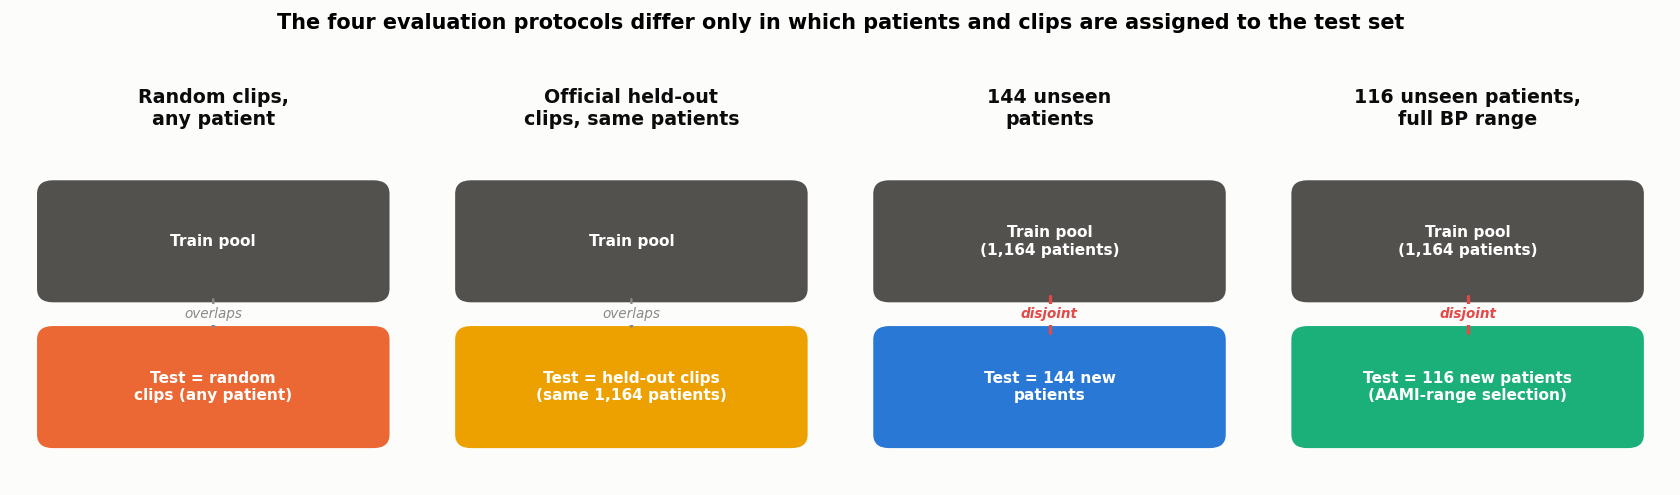
\includegraphics[width=0.92\textwidth]{paper_protocol_schematic.png}
\caption{Study design: the four evaluation protocols differ only in which patients and clips are assigned to the test set. Leaky and calibration-based test on previously seen patients; calibration-free and AAMI test on genuinely unseen ones.}
\label{fig:schematic}
\end{figure*}

\subsection{Models}
Five architectures were compared (Table~\ref{tab:arch}). Random Forest and Gradient Boosting were trained on 61 hand-crafted morphological and demographic features per clip. 1D-CNN (five convolutional blocks, 381{,}186 parameters) and ResNet1D (eight residual blocks across four stages, ResNet-18 style, 2.19M parameters) operated on the raw two-channel (ECG+PPG) waveform. The Transformer (1.41M parameters) followed the patch-10 self-attention architecture with demographic FiLM conditioning and a morphology-classification auxiliary head reported by Shen~\textit{et al.}~\cite{shen2026}, reproduced as closely as the published description allows: PPG-only input, per-clip z-score scaling, Adam optimizer (weight decay $1\mathrm{e}{-8}$, fixed learning rate $2\mathrm{e}{-5}$), batch size 32. Two deliberate deviations were made for cross-model budget parity: a single joint network predicting both SBP and DBP, and 50 training epochs rather than 100. Classical models and CNN/ResNet1D used AdamW (weight decay $1\mathrm{e}{-4}$) with a OneCycle learning-rate schedule; the CNN/ResNet1D primary calibration-free result used a schedule decoupled from total epoch count (fixed 20-epoch anneal) to avoid confounding ``more training'' with ``a differently shaped learning-rate curve.'' For every model, the best-validation-checkpoint was used for test-set scoring.

\begin{table}[!t]
\caption{Architecture and Training Configuration Summary}
\label{tab:arch}
\centering
\begin{tabular}{lccc}
\toprule
Model & Input & Params & Epochs/batch \\
\midrule
Random Forest & 61 features & 300 trees & n/a \\
Gradient Boosting & 61 features & 500 rounds & n/a \\
1D-CNN & raw ECG+PPG & 381{,}186 & 50 / 256 \\
ResNet1D & raw ECG+PPG & 2.19M & 50 / 256 \\
Transformer & raw PPG (z-score) & 1.41M & 50 / 32 \\
\bottomrule
\end{tabular}
\end{table}

\subsection{BP-Bin Weighting}
Training BP values in PulseDB are heavily skewed toward the normotensive range (71.7\% of training clips fall in 90--130~mmHg systolic; only 0.7\% exceed 170~mmHg). A weighted-loss correction, inversely proportional to each BP bin's training frequency (up to 24.7$\times$ for the rarest bin), was applied during training for every model and compared against an otherwise identical unweighted run.

\subsection{Personalization}
Per-subject personalization fit an affine correction, $\mathrm{corrected} = a \times \mathrm{predicted} + b$, from $k \in \{1,3,5,10,25\}$ of a held-out subject's own calibration-free test clips, with $a,b$ fit by least squares on those $k$ clips and applied to the subject's remaining clips. Because PulseDB's released calibration-free test file carries no session or case identifier, a genuinely cross-session test is not possible on this data; instead, two readings of ``first $k$ clips'' were compared. The \textit{naive} reading takes the first $k$ clips in storage order; storage order was confirmed uncorrelated with true recording time ($r=0.01$), so this selection scatters calibration clips across the session, placing an evaluation clip within roughly 3 minutes of a calibration clip on average. The \textit{chronological} reading sorts by the genuine segment-index field, takes the true earliest $k$ clips as calibration, and scores only clips later in the same session (approximately 70 minutes later on average) --- the strongest cross-time test this single-session dataset supports.

\subsection{Evaluation Metrics and Statistical Treatment}
MAE, mean error (bias), and error standard deviation (SD) were computed separately for SBP and DBP. AAMI pass/fail required bias within $\pm5$~mmHg and SD within 8~mmHg jointly; British Hypertension Society (BHS) grade \cite{obrien1990} required, for grade A, 60\% of predictions within 5~mmHg, 85\% within 10~mmHg, and 95\% within 15~mmHg. Three training seeds were run for calibration-free (all five models) and, to test whether the architecture-dependence finding is a seed artefact, for calibration-based and leaky protocols on the two convolutional architectures. Where three seeds exist, 95\% confidence intervals use a $t$-distribution ($df=2$); single-seed results are reported descriptively.

\subsection{Formal Definitions}
For a test set of $N$ clips with true values $y_i$ and predictions $\hat{y}_i$,
\begin{equation}
\mathrm{MAE} = \frac{1}{N}\sum_{i=1}^{N} \left| \hat{y}_i - y_i \right|, \quad
\mathrm{ME} = \frac{1}{N}\sum_{i=1}^{N} \left( \hat{y}_i - y_i \right)
\label{eq:mae}
\end{equation}
\begin{equation}
\mathrm{SD} = \sqrt{\frac{1}{N-1}\sum_{i=1}^{N} \left( (\hat{y}_i - y_i) - \mathrm{ME} \right)^2 }
\label{eq:sd}
\end{equation}
AAMI compliance requires $|\mathrm{ME}| \le 5$ and $\mathrm{SD} \le 8$~mmHg jointly, computed per target. The Transformer's training loss combines SBP/DBP regression with the auxiliary morphology-classification head via Kendall-style learnable homoscedastic uncertainty weighting \cite{shen2026}:
\begin{equation}
\mathcal{L} = \frac{1}{2\sigma_{bp}^2}\mathcal{L}_{bp} + \log\sigma_{bp} + \frac{1}{2\sigma_{shape}^2}\mathcal{L}_{shape} + \log\sigma_{shape}
\label{eq:kendall}
\end{equation}
where $\mathcal{L}_{bp}$ is Smooth-$L_1$ loss on standardised SBP/DBP targets, $\mathcal{L}_{shape}$ is cross-entropy on the binary morphology label, and $\log\sigma_{bp},\log\sigma_{shape}$ are learned jointly with the network weights. The $k$-shot personalization correction, for calibration clips indexed $c \in C_k$ ($|C_k|=k$) of a held-out subject, fits
\begin{equation}
(a^\ast, b^\ast) = \operatorname*{arg\,min}_{a,b} \sum_{c \in C_k} \left( a\,\hat{y}_c + b - y_c \right)^2
\label{eq:affine}
\end{equation}
by ordinary least squares and applies $\hat{y}'_i = a^\ast \hat{y}_i + b^\ast$ to the subject's remaining clips $i \notin C_k$. The physiological ceiling (Table~\ref{tab:ceiling}) is the special case of Eq.~\eqref{eq:affine} fit with $C_k$ equal to the subject's \emph{entire} true-labelled test pool, representing the best any constant per-subject offset could achieve if calibration labels were unlimited and noise-free.

\subsection{Implementation and Training Infrastructure}
Classical models (Random Forest, Gradient Boosting) were trained on CPU. Deep models (1D-CNN, ResNet1D, Transformer) were trained on a mix of cloud GPU instances (NVIDIA T4-class, via free-tier notebook services, and an institutional workstation GPU) as availability allowed across the study's timeline; the specific accelerator used does not affect reported accuracy, since every number in this paper is read from a saved checkpoint's test-set evaluation rather than from training-time logs. Per-epoch wall-clock time for the Transformer ranged from approximately 280 to 440~seconds depending on the specific GPU in use at the time, giving a full 50-epoch run on the order of 4--6 hours; the complete 13-run Transformer sweep (all seeds, all protocols) plus six domain-shift evaluations completed in approximately 2.3~days of wall-clock time on the fastest accelerator used. All training and evaluation code, including the exact configuration for every run reported here, is released alongside this manuscript (see Data and Code Availability).

\section{Results}

\subsection{The Calibration-Free Gap Is Large and Architecture-Dependent}
Table~\ref{tab:canonical} reports MAE for every model under every protocol. Relative to the average of leaky and calibration-based performance, calibration-free accuracy was 1.09 to 2.28 times worse, depending on architecture (Fig.~\ref{fig:gap}). The Transformer showed the smallest gap (1.09$\times$: 14.13~mmHg seen-patient average versus 15.44~mmHg calibration-free) --- not because it is uniformly most accurate (it is in fact worst of the five on calibration-based specifically, 13.80~mmHg) --- but because it does not benefit from already-seen patients to the same degree the other four architectures do. ResNet1D showed the largest gap (2.28$\times$: 6.12~mmHg versus 13.96~mmHg). This architecture-dependence held under a three-seed check on the two convolutional architectures (SD 0.25--0.90~mmHg across seeds, an order of magnitude smaller than the gaps separating architectures).

\begin{table*}[!t]
\caption{Mean Absolute Error (SBP / DBP, mmHg) by Model and Protocol}
\label{tab:canonical}
\centering
\begin{tabular}{lccccc}
\toprule
Model & calfree (w) & calfree (u) & calbased & leaky & AAMI \\
\midrule
Random Forest & 12.77/8.39* & 12.81/8.59* & 7.14/4.11 & 7.47/4.34 & 19.67/12.24 \\
Gradient Boosting & 14.67/8.98* & 12.76/8.33* & 10.20/6.03 & 10.29/6.13 & 17.44/11.14 \\
1D-CNN & 14.89/9.04\textdagger & 13.01/8.34 & 10.15/6.55* & 10.36/6.80* & 16.53/11.20 \\
ResNet1D & 13.94/8.94\textdagger & 13.21/8.53 & 6.71/4.26* & 6.41/4.03* & 17.70/11.40 \\
Transformer & 15.81/8.71* & 12.89/7.91* & 13.90/8.06* & 13.90/7.96* & 17.03/10.15 \\
\bottomrule
\end{tabular}
\\[2pt]
\raggedright\footnotesize * = three-seed mean. \textdagger\ = single schedule-fixed run (CNN/ResNet1D calfree-weighted only), not seed-averaged. (w) = BP-bin weighted (primary); (u) = unweighted (comparable to prior published numbers). Unmarked cells are single seed-0 runs.
\end{table*}

\begin{figure*}[!t]
\centering
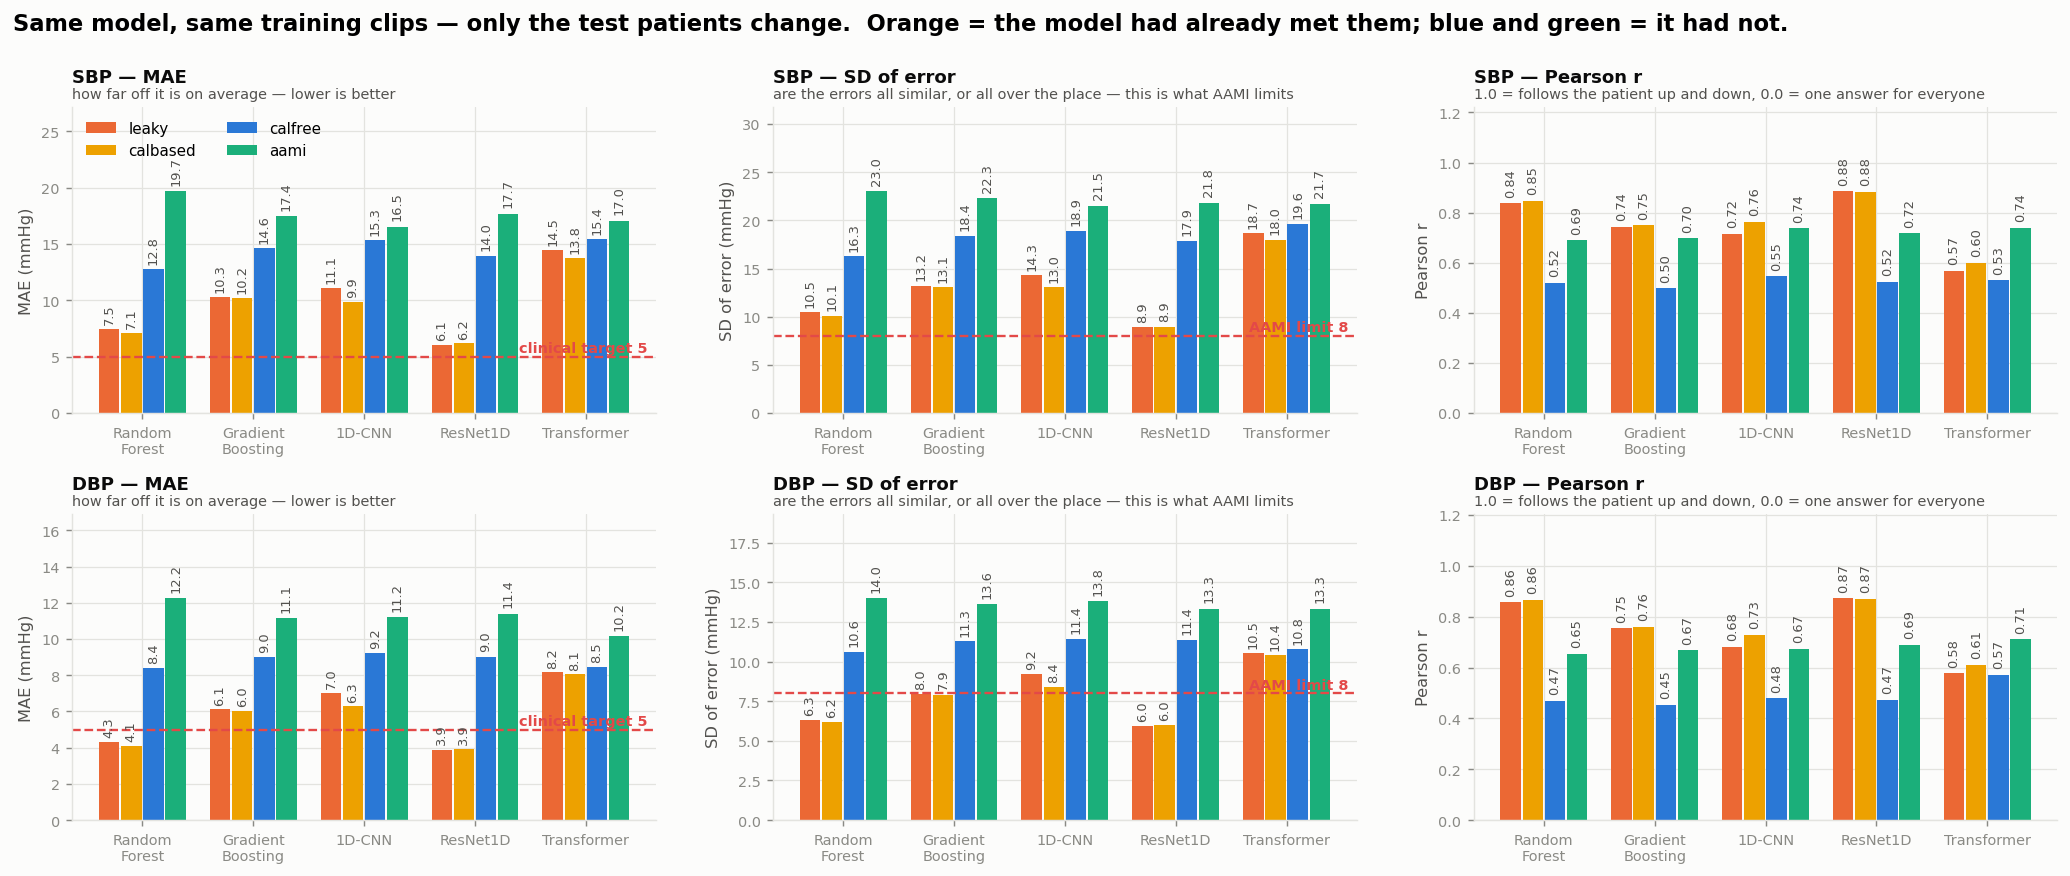
\includegraphics[width=0.92\textwidth]{1_leakage_gap.png}
\caption{Known-patient (leaky/calibration-based average) versus calibration-free accuracy, all five models, SBP and DBP. Orange/yellow bars test on previously seen patients; blue/aqua bars test on unseen patients.}
\label{fig:gap}
\end{figure*}

\subsection{Full Clinical Metric Set}
Table~\ref{tab:clinical} reports correlation, AAMI pass/fail, and BHS grade for the calibration-free (weighted) result. Pearson $r$ is modest across the board (0.45--0.57); the Transformer's DBP correlation (0.57) is the highest of any model/target pair, consistent with it carrying the least calibration-free penalty overall. Every model fails BHS grade D (the lowest) and AAMI on calibration-free, for both targets.

\begin{table*}[!t]
\caption{Full Clinical Metric Set, Calibration-Free (Weighted)}
\label{tab:clinical}
\centering
\begin{tabular}{lcccccc}
\toprule
Model & SBP $r$ & SBP AAMI & SBP BHS & DBP $r$ & DBP AAMI & DBP BHS \\
\midrule
Random Forest & 0.518 & FAIL & D & 0.468 & FAIL & D \\
Gradient Boosting & 0.497 & FAIL & D & 0.454 & FAIL & D \\
1D-CNN & 0.546 & FAIL & D & 0.479 & FAIL & D \\
ResNet1D & 0.525 & FAIL & D & 0.473 & FAIL & D \\
Transformer & 0.530 & FAIL & D & 0.570 & FAIL & D \\
\bottomrule
\end{tabular}
\end{table*}

For completeness beyond the calibration-free summary in Table~\ref{tab:clinical}, Fig.~\ref{fig:compliance} reproduces the full clinical-compliance matrix across all four protocols, all five models, both targets, and both AAMI and BHS grading. The pattern is consistent across the matrix: leaky and calibration-based protocols pass AAMI for DBP on four of five models (ResNet1D passing with BHS grade A on both), while calibration-free and AAMI protocols fail AAMI for every model on both targets, reinforcing that the primary finding of this study --- the seen/unseen protocol distinction, not architecture choice, is the dominant driver of pass/fail status --- holds target-by-target and not only in the MAE-only summary of Section~IV-A.

\begin{figure*}[!t]
\centering
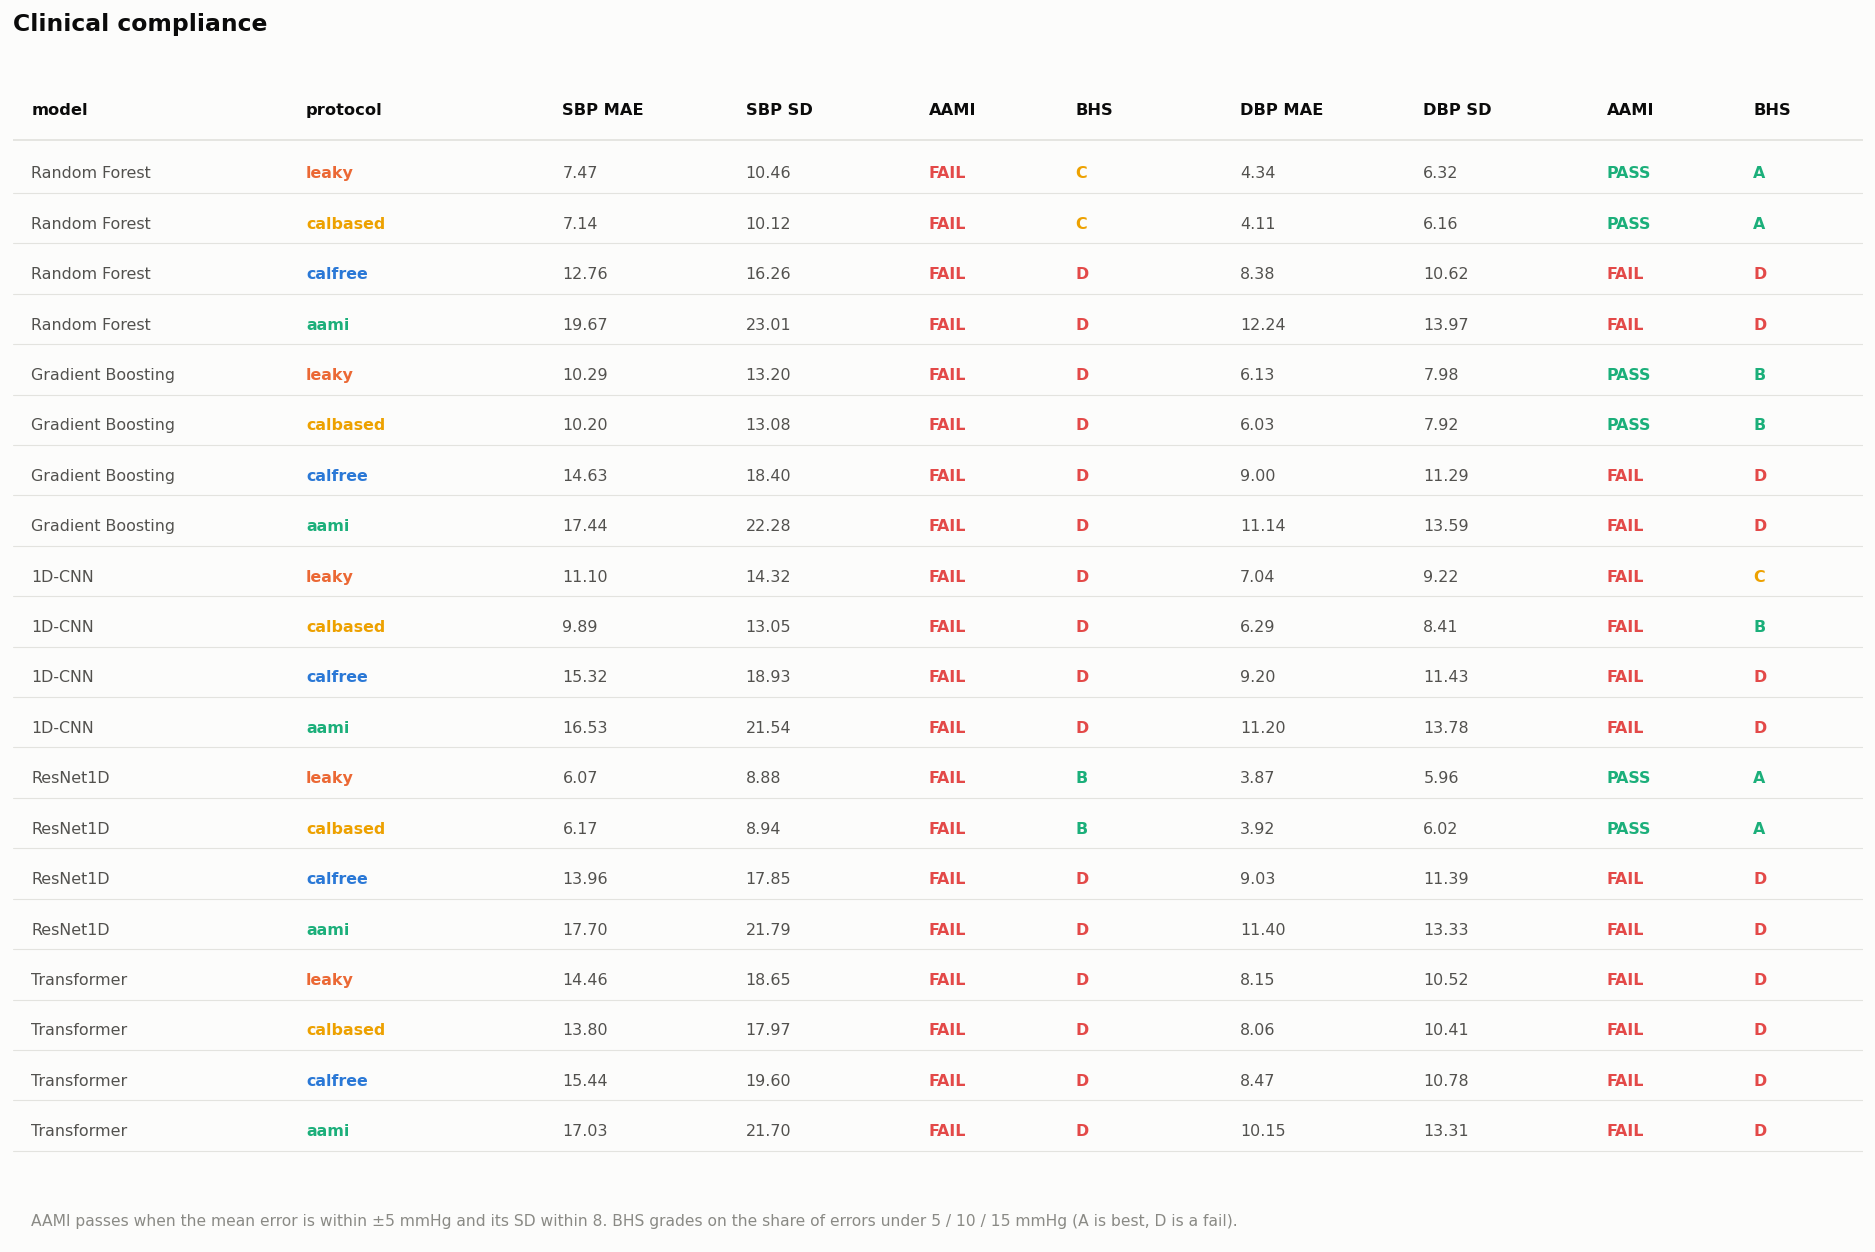
\includegraphics[width=0.85\textwidth]{2_compliance.png}
\caption{Full clinical compliance matrix: SBP/DBP MAE, SD, AAMI pass/fail, and BHS grade, all five models, all four protocols.}
\label{fig:compliance}
\end{figure*}

\subsection{BP-Bin Weighting: Cost and Benefit}
BP-bin weighting's effect was architecture-specific rather than uniformly beneficial (Fig.~\ref{fig:weighting}). It cost essentially nothing for Random Forest ($-0.18$~mmHg overall) while recovering 4.05~mmHg in the above-170-mmHg band; it cost the Transformer the most overall ($+2.77$~mmHg) while recovering the second-most in that band (16.41~mmHg, behind only the CNN's 17.52~mmHg). Below 130~mmHg systolic (72\% of test clips), the unweighted model was frequently equal or better; above 150~mmHg, weighting's benefit was consistent across every architecture. No single weighted/unweighted choice dominated, which is why both are reported throughout.

\begin{figure*}[!t]
\centering
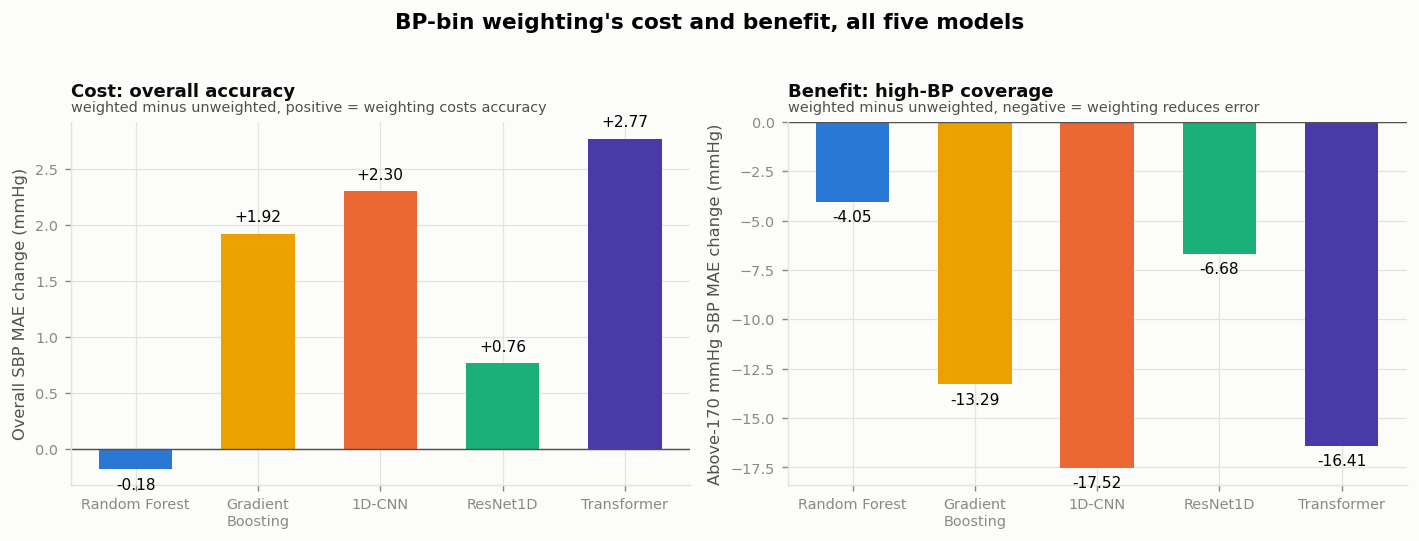
\includegraphics[width=0.92\textwidth]{paper_weighting_all_models.png}
\caption{BP-bin weighting's cost (overall SBP MAE change) and benefit (above-170~mmHg SBP MAE change), weighted minus unweighted training, all five models.}
\label{fig:weighting}
\end{figure*}

\subsection{Against the Literature}
Fig.~\ref{fig:literature} compares this study's calibration-free, unweighted results against four prior studies on the same VitalDB subset. The Transformer's unweighted result (12.67~mmHg SBP, three-seed mean 12.89, SD 0.32) was the closest match to the current best published number, Shen~\textit{et al.}'s demographic-conditioned transformer (12.17~mmHg) \cite{shen2026} --- ahead of every other architecture tested here and of Moulaeifard~\textit{et al.}'s XResNet1d101 benchmark (12.70~mmHg) \cite{moulaeifard2025}. The 1D-CNN's unweighted result (13.01~mmHg, three-seed mean 13.04, SD 0.12) was close behind. The gap between four years of published architecture progress on this benchmark (roughly 12.17 to 13.67~mmHg across the four prior studies compared here) is smaller than the 1.09$\times$--2.28$\times$ gap this study measures from evaluation protocol alone on a single architecture.

\begin{figure}[!t]
\centering
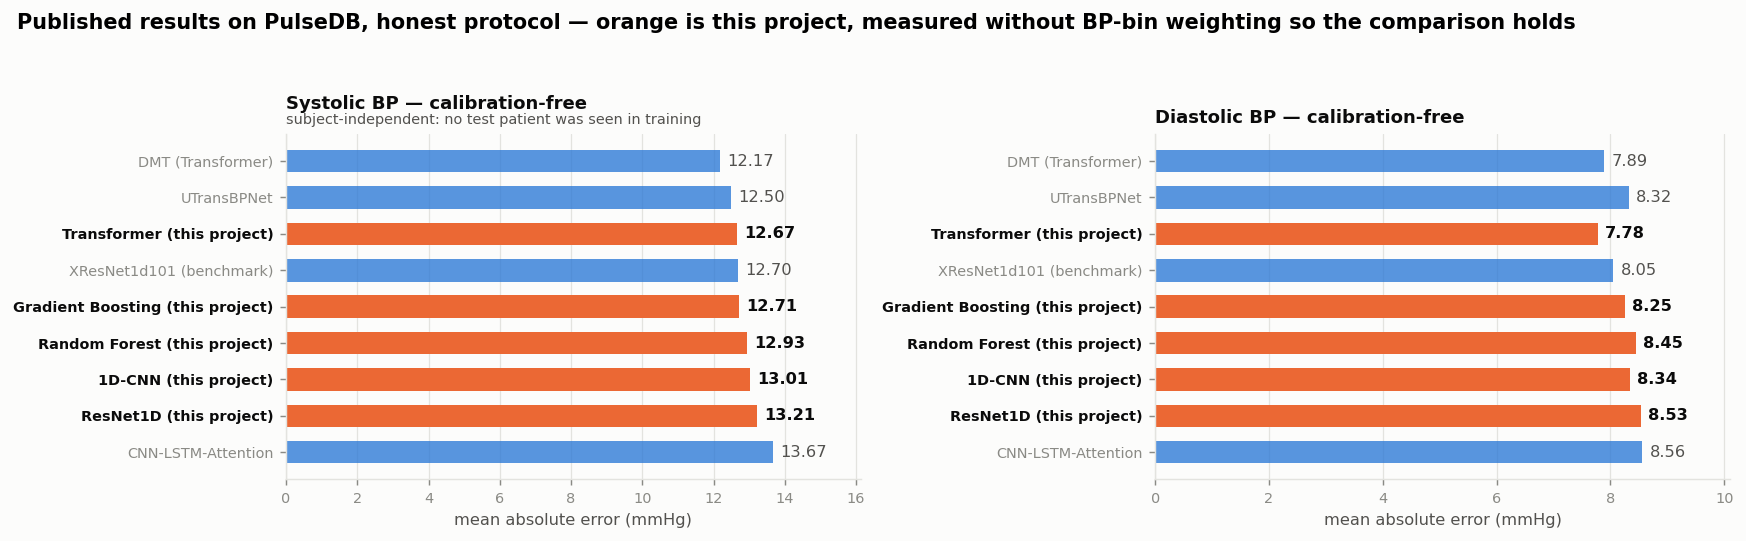
\includegraphics[width=0.48\textwidth]{01_calibration_free_comparison.png}
\caption{Calibration-free SBP MAE, this study (orange, unweighted) against four prior studies on the same PulseDB VitalDB subset (blue).}
\label{fig:literature}
\end{figure}

\subsection{AAMI Sampling-Coverage Check}
Table~\ref{tab:aami} checks whether the calibration-free split itself satisfies AAMI/ISO~81060-2's own sampling requirement for reference-BP coverage. It does not: the split fails three of four BP-range criteria for both SBP and DBP (e.g., only 1.5\% of subjects reach 160~mmHg systolic, against a 5\% requirement). PulseDB's AAMI-specific split, built explicitly to span the full clinical range, passes every criterion.

\begin{table}[!t]
\caption{AAMI/ISO 81060-2 Sampling-Coverage Check}
\label{tab:aami}
\centering
\footnotesize
\begin{tabular}{lcc}
\toprule
Requirement & calfree\_test (144) & aami\_test (116) \\
\midrule
$N \geq 85$ & PASS (144) & PASS (116) \\
SBP $\leq$10 in $\geq$5\% & PASS (21.3\%) & PASS (15.6\%) \\
SBP $\geq$160 in $\geq$5\% & FAIL (1.5\%) & PASS (21.5\%) \\
SBP $\geq$140 in $\geq$20\% & FAIL (10.3\%) & PASS (42.6\%) \\
DBP $\leq$60 in $\geq$5\% & PASS (41.2\%) & PASS (24.5\%) \\
DBP $\geq$100 in $\geq$5\% & FAIL (0.3\%) & PASS (10.5\%) \\
DBP $\geq$85 in $\geq$20\% & FAIL (4.1\%) & PASS (31.5\%) \\
\bottomrule
\end{tabular}
\end{table}

\subsection{External, Label-Free Wearable Check}
On PPG-DaLiA (Fig.~\ref{fig:shift}), every model's mean predicted SBP exceeded the healthy-adult norm, and models still separated individuals by 2.1--9.6~mmHg (true spread: 11.8~mmHg). The fraction of the apparent shift attributable to BP-bin weighting ranged from 2\% (Transformer) to 40\% (Gradient Boosting) across four of five models; ResNet1D was a reversed outlier, where weighting reduced rather than enlarged the shift. Heart-rate MAE, the only ground-truth metric on this dataset, was 13.06~bpm in low-motion activity segments (sitting, lunch, working, driving) and 33.35~bpm in high-motion segments (cycling, stairs, walking, table soccer, transient) using this study's generic pulse detector, against 8.69~bpm reported by Reiss~\textit{et al.}~\cite{reiss2019} using a dedicated denoiser on the same data.

Table~\ref{tab:plausible} reports a second, independent label-free check: the fraction of each model's PPG-DaLiA predictions that fall outside physiologically plausible clinical range (SBP outside 70--200~mmHg or DBP outside 40--120~mmHg). No model ever predicts DBP above SBP for the same clip. Beyond that, the rate of out-of-range predictions spans two orders of magnitude by architecture, from 0.5\% (Transformer) to 29.7\% (Gradient Boosting); the two classical ensembles produce an implausible prediction on roughly one clip in four to one in three, while the three deep models stay under 3.4\%. This is a plausibility check rather than an accuracy check --- it does not require true labels and cannot confirm a prediction is correct, only flag predictions that are certainly wrong --- and it reinforces Section~IV-M's finding that representation choice affects out-of-distribution behaviour beyond what calibration-free MAE alone shows.

\begin{table}[!t]
\caption{Physiologically Implausible Predictions on PPG-DaLiA (\% of Clips)}
\label{tab:plausible}
\centering
\begin{tabular}{lccc}
\toprule
Model & SBP out of range & DBP out of range & Any \\
\midrule
Random Forest & 0.0\% & 27.2\% & 27.2\% \\
Gradient Boosting & 13.8\% & 25.7\% & 29.7\% \\
1D-CNN & 2.0\% & 2.2\% & 3.4\% \\
ResNet1D & 0.0\% & 0.8\% & 0.8\% \\
Transformer & 0.3\% & 0.5\% & 0.5\% \\
\bottomrule
\end{tabular}
\\[2pt]
\raggedright\footnotesize Plausible range: SBP $\in[70,200]$~mmHg, DBP $\in[40,120]$~mmHg. DBP $>$ SBP on the same clip: 0.0\% for every model.
\end{table}

\begin{figure*}[!t]
\centering
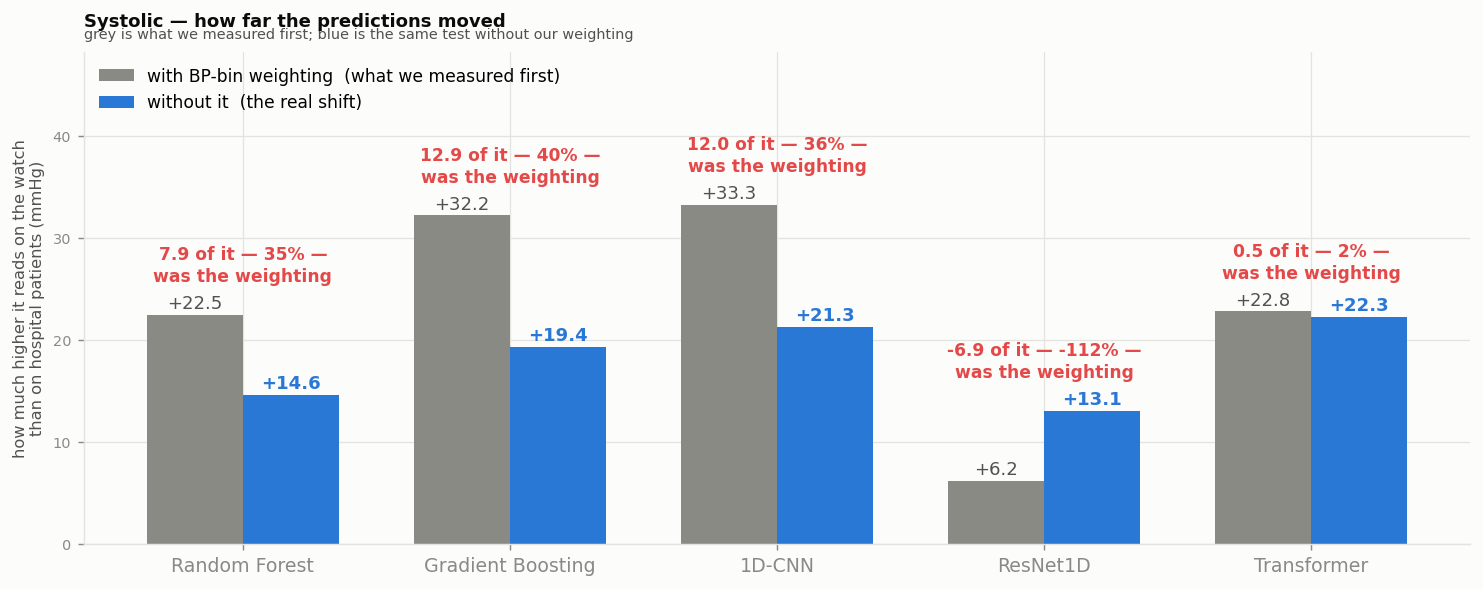
\includegraphics[width=0.92\textwidth]{3_shift_amount.png}
\caption{Predicted SBP shift from PulseDB to PPG-DaLiA, weighted versus unweighted training, all five models.}
\label{fig:shift}
\end{figure*}

\subsection{Domain-Shift Collapse Check}
A model that collapses to predicting a single value for every subject on a new device would still show a nonzero ``shift'' in Fig.~\ref{fig:shift} without that shift reflecting any genuine signal. This was checked directly by comparing each model's between-subject prediction spread on PulseDB against its spread on PPG-DaLiA (Fig.~\ref{fig:collapse}). Random Forest's between-subject SBP spread fell from 8.0~mmHg on PulseDB's hospital patients to 2.1~mmHg on the watch data, the sharpest collapse of the five models, while still remaining above zero, indicating it retains some between-subject discrimination rather than converging to one constant output. Weighted and unweighted training produced near-identical collapse behaviour for every model, confirming that collapse is a property of the device/population shift itself rather than of the BP-bin weighting correction.

\begin{figure*}[!t]
\centering
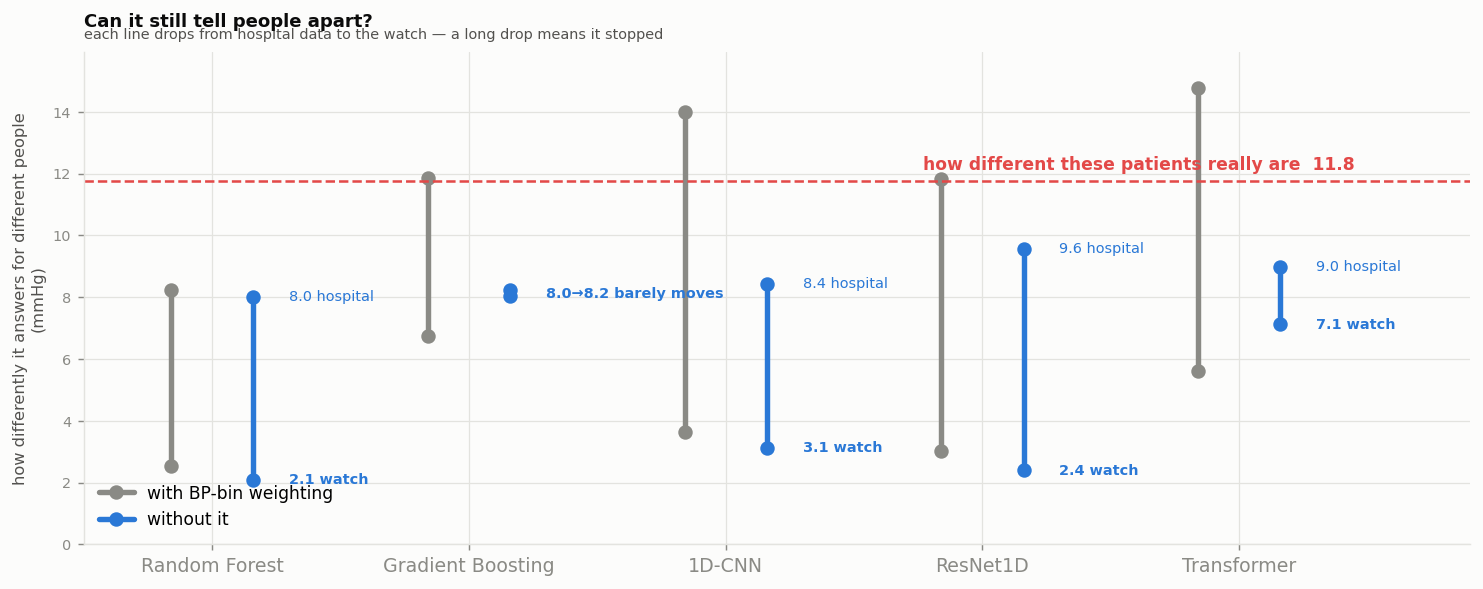
\includegraphics[width=0.92\textwidth]{3_shift_collapse.png}
\caption{Between-subject prediction spread, PulseDB (hospital patients) versus PPG-DaLiA (watch volunteers), all five models. A collapse toward zero spread would indicate the model answers near-identically for every subject on the new device; all five models retain nonzero, if reduced, spread.}
\label{fig:collapse}
\end{figure*}

\subsection{Personalization: Diastolic Recovers, Systolic Does Not}
Table~\ref{tab:pers} and Fig.~\ref{fig:pers} report personalization results. Under the naive (storage-order) split, 25 clips reduced diastolic MAE by 20--51\% across the five models, and every model passed AAMI's diastolic criterion from roughly five calibration clips onward, coming within 0.3~mmHg of each architecture's physiological ceiling (Table~\ref{tab:ceiling}). Across all five models, 33--41\% of raw SBP error and 40--46\% of raw DBP error was fixable, constant per-subject offset; the remainder reflects within-subject BP variability, since systolic BP varies more within one subject's own recording (SD 13.9~mmHg, 1D-CNN) than between subjects (11.8~mmHg).

\begin{table*}[!t]
\caption{Personalization Ceiling: Raw MAE vs.\ Oracle Offset}
\label{tab:ceiling}
\centering
\begin{tabular}{lcccc}
\toprule
Model & SBP raw$\to$oracle & SBP recov. & DBP raw$\to$oracle & DBP recov. \\
\midrule
Random Forest & 12.76$\to$8.48 & 33\% & 8.38$\to$4.98 & 41\% \\
Gradient Boosting & 14.63$\to$8.77 & 40\% & 9.00$\to$5.15 & 43\% \\
1D-CNN & 15.32$\to$9.03 & 41\% & 9.20$\to$5.00 & 46\% \\
ResNet1D & 13.96$\to$9.01 & 35\% & 9.03$\to$5.46 & 40\% \\
Transformer & 15.44$\to$9.34 & 39\% & 8.47$\to$4.94 & 42\% \\
\bottomrule
\end{tabular}
\end{table*}

Why the ceiling sits near 7--9~mmHg rather than 1--2~mmHg follows directly from how within- and between-subject variance compare on this benchmark. Writing $\sigma^2_{\mathrm{within}}$ for the average variance of a subject's own SBP readings around that subject's mean, and $\sigma^2_{\mathrm{between}}$ for the variance of subject means around the population mean, a constant per-subject offset can in principle remove all of $\sigma^2_{\mathrm{between}}$ but none of $\sigma^2_{\mathrm{within}}$: the best any such correction can achieve is bounded below by $\sigma_{\mathrm{within}}$ itself. For the 1D-CNN, $\sigma_{\mathrm{within}} = 13.9$~mmHg exceeds $\sigma_{\mathrm{between}} = 11.8$~mmHg, so more than half of the total variance a constant correction would need to explain is, by construction, outside what a constant correction can reach --- consistent with the oracle ceiling recovering only 33--41\% of raw SBP error (Table~\ref{tab:ceiling}) rather than approaching 100\%. Closing the remainder would require modelling beat-to-beat or short-term within-subject dynamics, which a per-subject constant offset cannot represent regardless of how many calibration clips are used to fit it.

Under the chronological split, the picture changed substantially: diastolic MAE still improved (e.g., Random Forest: 8.38 to 7.32~mmHg), but no model met AAMI's spread criterion at any calibration size, for any architecture. Bias stayed under 2~mmHg throughout, so the shortfall reflects error spread specifically. This is consistent with the naive split allowing the correction to exploit short-term signal continuity (an average 3-minute calibration-to-evaluation gap) that does not persist across the chronological split's roughly 70-minute gap. Table~\ref{tab:chron-sweep} gives the full chronological-split sweep underlying this claim: SDE never approaches AAMI's 8~mmHg spread bound at any tested $k$, for any model, including the largest calibration set tested ($k$=25, best case 8.75~mmHg, Transformer).

\begin{table*}[!t]
\caption{Chronological-Split DBP MAE / SDE Across the Full Calibration-Size Sweep (mmHg)}
\label{tab:chron-sweep}
\centering
\begin{tabular}{lccccc}
\toprule
Model & $k$=1 & $k$=3 & $k$=5 & $k$=10 & $k$=25 \\
\midrule
Random Forest & 9.58/12.74 & 11.97/18.96 & 9.46/12.68 & 8.65/11.86 & 7.32/9.68 \\
Gradient Boosting & 9.11/11.84 & 13.11/27.74 & 9.23/12.32 & 7.95/10.53 & 7.11/9.47 \\
1D-CNN & 10.11/13.30 & 11.51/17.35 & 9.39/12.89 & 8.20/10.99 & 7.25/9.75 \\
ResNet1D & 10.54/13.59 & 11.10/15.61 & 9.41/12.68 & 8.44/11.17 & 7.38/9.47 \\
Transformer & 9.60/12.59 & 10.38/14.81 & 8.38/11.23 & 7.60/10.08 & 6.68/8.75 \\
\bottomrule
\end{tabular}
\\[2pt]
\raggedright\footnotesize Cells are MAE/SDE. AAMI requires SDE $\le 8$~mmHg; no cell meets this. Every model fails AAMI at every $k$ under the chronological split.
\end{table*}

\begin{table}[!t]
\caption{Diastolic MAE (mmHg), $k$=0 vs.\ $k$=25}
\label{tab:pers}
\centering
\footnotesize
\begin{tabular}{lccccc}
\toprule
Model & $k$=0 & naive & A. & chron. & A. \\
\midrule
Random Forest & 8.38 & 4.81 & PASS & 7.32 & FAIL \\
Gradient Boosting & 9.00 & 4.74 & PASS & 7.11 & FAIL \\
1D-CNN & 9.20 & 4.51 & PASS & 7.25 & FAIL \\
ResNet1D & 9.03 & 4.83 & PASS & 7.38 & FAIL \\
Transformer & 8.47 & 4.40 & PASS & 6.68 & FAIL \\
\bottomrule
\end{tabular}
\\[2pt]
\raggedright\footnotesize A. = AAMI status at $k$=25.
\end{table}

\begin{figure*}[!t]
\centering
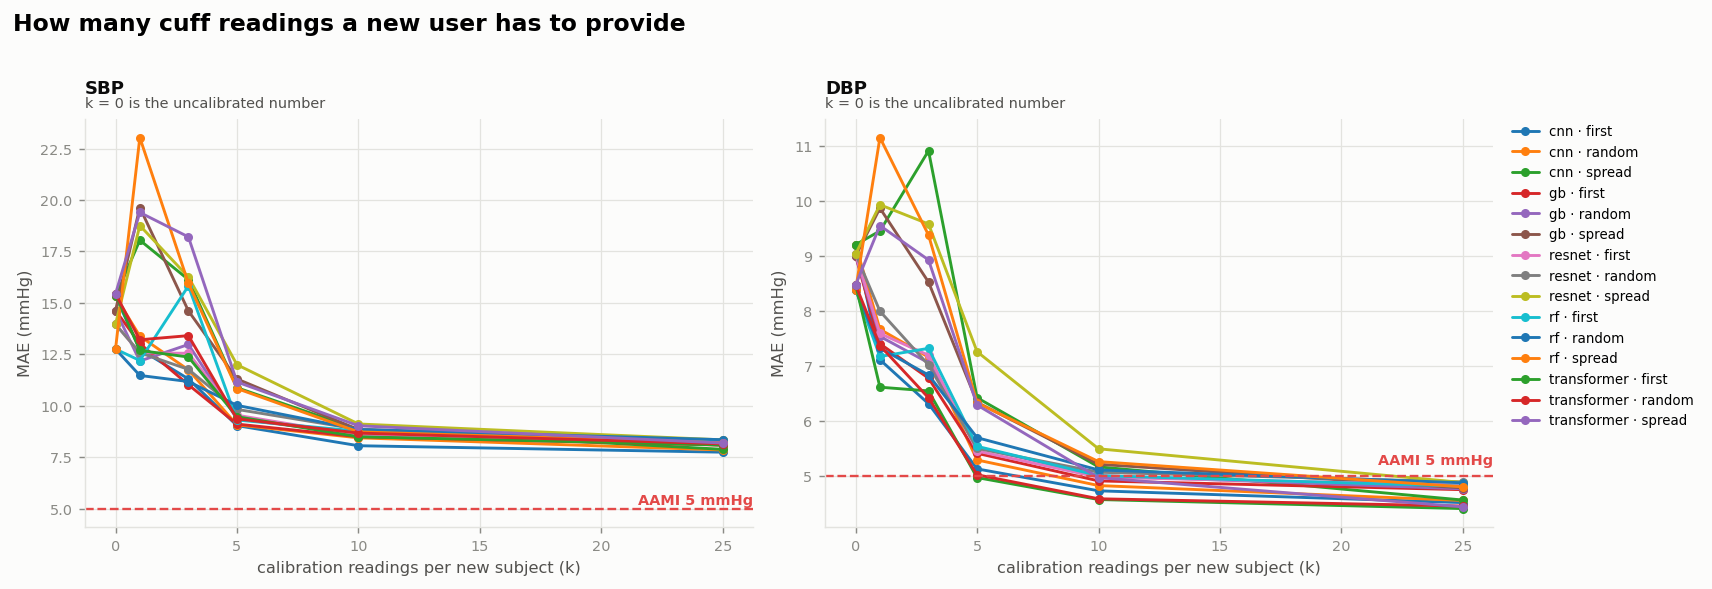
\includegraphics[width=0.92\textwidth]{5_personalization.png}
\caption{Error reduction as a function of calibration-clip count ($k=0$--25), all five models. Most recoverable error is gone by $k=5$; two models show a brief worsening at $k=3$, indicating 2--3 clips is too few to fit a stable correction.}
\label{fig:pers}
\end{figure*}

\subsection{Isolating the Learning-Rate-Schedule Confound}
A OneCycle learning-rate schedule's shape is a function of the total epoch budget: at a given epoch, a 20-epoch run and a 50-epoch run are at different points of their respective annealing curves, so comparing a 20-epoch result against a 50-epoch result on the same architecture conflates ``more training'' with ``a differently shaped learning-rate trajectory.'' To isolate this, CNN and ResNet1D were re-run with a decoupled schedule-length parameter fixed at 20 epochs regardless of the total epoch budget, so the first 20 epochs of a 20-epoch and a 50-epoch run are optimized identically. Table~\ref{tab:onecycle} reports the result. For the CNN, closing the confound recovers nearly the entire apparent degradation from more training (14.89 vs.\ the original 14.86/9.01) --- most of what looked like ``50 epochs overfits'' was schedule shape, not genuinely more training. For ResNet1D, the recovery is partial: DBP returns almost exactly to the 20-epoch value (8.94 vs.\ 8.97), but SBP remains close to the confounded 50-epoch value (13.94 vs.\ 13.96, both above the original 13.58), indicating SBP's degradation at 50 epochs reflects genuine overfitting rather than a schedule artefact for this architecture specifically.

\begin{table}[!t]
\caption{Closing the Learning-Rate-Schedule Confound (SBP / DBP, mmHg)}
\label{tab:onecycle}
\centering
\begin{tabular}{lccc}
\toprule
Model & 20-ep. original & 50-ep. confounded & 50-ep. fixed \\
\midrule
1D-CNN & 14.86/9.01 & 15.32/9.20 & 14.89/9.04 \\
ResNet1D & 13.58/8.97 & 13.96/9.03 & 13.94/8.94 \\
\bottomrule
\end{tabular}
\end{table}

Fig.~\ref{fig:training} shows the mechanism underlying this confound directly. Validation loss stops improving within the first 5--15 epochs for both CNN and ResNet1D, while training loss continues falling well past that point --- the model is memorising its own training clips rather than learning anything that generalises further. This alone would not hurt the reported result, since best-validation-checkpoint selection (Section~III-C) picks the best epoch regardless of how many more follow; what actually changes the outcome is that the learning-rate curve up to any given epoch is not the same shape in a 20-epoch run as in a 50-epoch run, so the 50-epoch run's best checkpoint was reached via a different, not merely longer, optimisation path.

\begin{figure*}[!t]
\centering
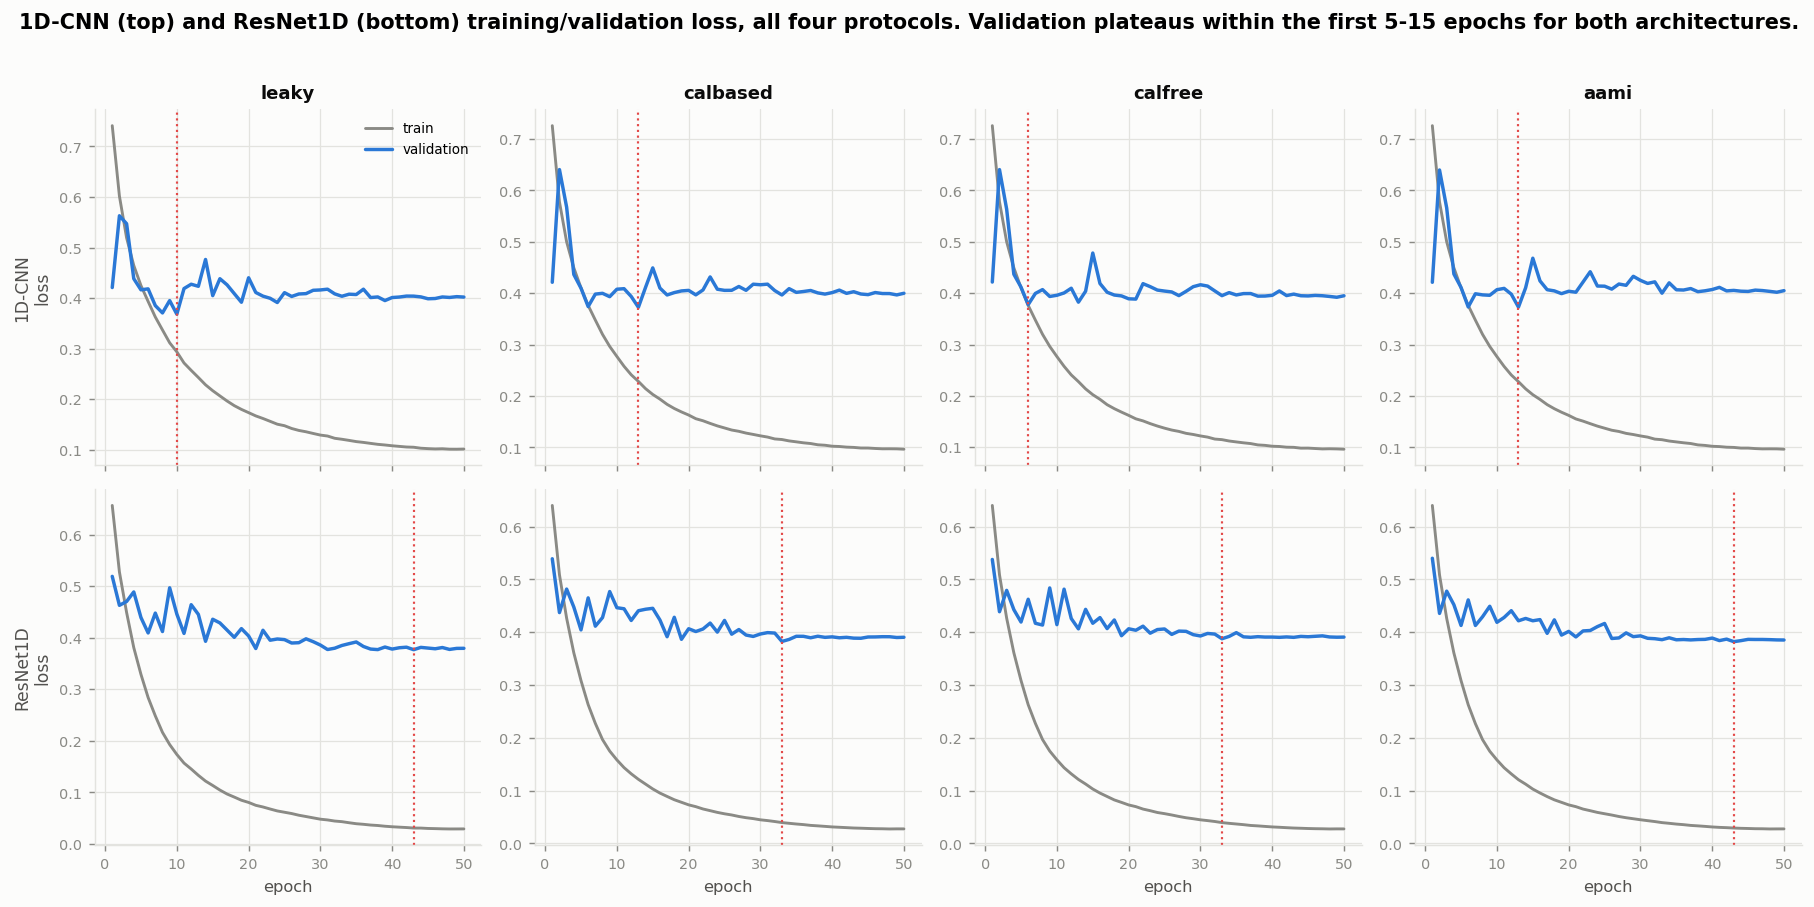
\includegraphics[width=0.92\textwidth]{paper_training_curves_cnn_resnet.png}
\caption{1D-CNN (top) and ResNet1D (bottom) training and validation loss, all four protocols. Validation loss plateaus within the first 5--15 epochs for both architectures while training loss continues to fall, illustrating the memorisation effect underlying the schedule confound of Section~IV-H. ResNet1D's best-validation epoch (dotted line) lands later than the CNN's because its validation loss is noisier once plateaued, not because it keeps improving.}
\label{fig:training}
\end{figure*}

\subsection{Seed Variance, Full Breakdown}
Table~\ref{tab:seeds} reports the complete three-seed breakdown underlying every confidence interval in this study, for the calibration-free protocol under both weighting conditions. Every per-target standard deviation is under 0.33~mmHg, an order of magnitude smaller than the differences this study's headline findings are built on, supporting the claim that those findings are not single-seed artefacts.

\begin{table*}[!t]
\caption{Seed Variance, Calibration-Free, Weighted and Unweighted (SBP / DBP, mmHg)}
\label{tab:seeds}
\centering
\begin{tabular}{llcccc}
\toprule
Model & Weighting & Seed 0 & Seed 1 & Seed 2 & SBP / DBP SD \\
\midrule
Random Forest & weighted & 12.76/8.38 & 12.79/8.37 & 12.77/8.41 & 0.016/0.014 \\
Random Forest & unweighted & 12.93/8.45 & 12.74/8.64 & 12.77/8.69 & 0.084/0.105 \\
Gradient Boosting & weighted & 14.63/9.00 & 14.76/8.94 & 14.62/9.00 & 0.065/0.028 \\
Gradient Boosting & unweighted & 12.71/8.25 & 12.73/8.36 & 12.84/8.38 & 0.060/0.058 \\
1D-CNN & weighted & 15.32/9.20 & 14.83/9.19 & 14.96/9.19 & 0.205/0.007 \\
1D-CNN & unweighted & 13.01/8.34 & 12.91/8.31 & 13.20/8.99 & 0.120/0.315 \\
ResNet1D & weighted & 13.96/9.03 & 14.01/9.29 & 13.68/8.79 & 0.145/0.205 \\
ResNet1D & unweighted & 13.21/8.53 & 13.71/9.16 & 13.35/9.17 & 0.211/0.297 \\
Transformer & weighted & 15.44/8.47 & 15.99/9.00 & 16.01/8.65 & 0.322/0.268 \\
Transformer & unweighted & 12.67/7.78 & 13.25/8.14 & 12.74/7.80 & 0.319/0.203 \\
\bottomrule
\end{tabular}
\end{table*}

\subsection{Statistical Power and Multiple Comparisons}
This study reports confidence intervals only where three seeds exist (Table~\ref{tab:seeds}), using a $t$-distribution with $df=2$; the resulting intervals are consequently wide relative to what a larger seed count would give, and should be read as a check against gross seed instability rather than as a tight estimate. The great majority of comparisons made across this paper --- weighted versus unweighted (every model, every protocol), naive versus chronological personalization, schedule-confounded versus schedule-fixed training, and the leaky/calibration-based results for the two classical models --- are single-run comparisons reported descriptively, without an associated interval. Counting conservatively, this study makes on the order of $5~\mathrm{models} \times 4~\mathrm{protocols} \times 2~\mathrm{(weighted/unweighted)} \times 5~\mathrm{(}k\mathrm{\ values)} \approx 200$ distinct numerical comparisons; none of the confidence intervals reported are corrected for this multiplicity (e.g., via a Bonferroni or false-discovery-rate adjustment). This is stated explicitly here, consistent with the reporting-transparency recommendation of Elgendi~\textit{et al.}~\cite{elgendi2024}, rather than left for a reader to infer. The two findings this study treats as its primary claims --- the architecture-dependence of the calibration-free gap, and the naive-versus-chronological personalization gap --- are each supported by a direct, matched comparison under otherwise identical conditions rather than by a single corrected $p$-value, which is the more conservative basis available given the single-seed status of most secondary comparisons.

\subsection{Agreement Analysis}
Fig.~\ref{fig:bland} summarises Bland--Altman bias and 95\% limits of agreement for all five models across all four protocols, the secondary agreement metric requested alongside MAE. For every model, the limits of agreement widen from leaky through calibration-based and calibration-free to AAMI, and bias tilts negative under AAMI across all five architectures --- each model pulling every unfamiliar, extreme-range patient toward the population average, a pattern invisible in a single pooled MAE number but directly visible here. The direction of this bias tilt is consistent across classical and deep models alike, indicating it is a property of the evaluation protocol rather than of any one architecture. ResNet1D's limits of agreement are the narrowest of the five models on leaky and calibration-based (\textpm17~mmHg SBP), consistent with it also having the lowest MAE on those two protocols (Table~\ref{tab:canonical}); the two properties move together here rather than dissociating.

\begin{figure*}[!t]
\centering
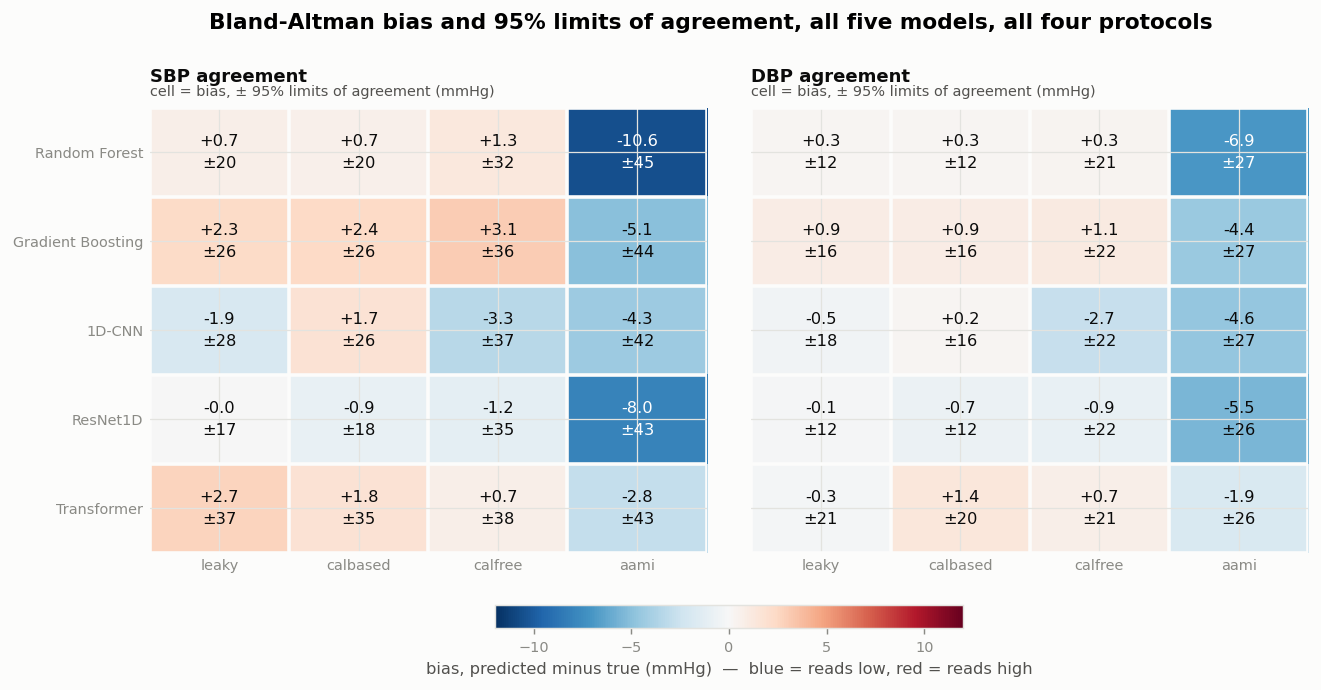
\includegraphics[width=0.92\textwidth]{paper_bland_altman_all_models.png}
\caption{Bland--Altman bias and 95\% limits of agreement, all five models, all four protocols, both targets. Each cell reports bias $\pm$ the limits of agreement; colour encodes bias (blue = reads low, red = reads high). Bias tilts negative (blue) under AAMI for every model; limits widen from leaky to AAMI for every model.}
\label{fig:bland}
\end{figure*}

\subsection{Feature Representation: Classical vs.\ Raw Waveform}
Table~\ref{tab:features} isolates representation choice from architecture depth by comparing Random Forest's 61 hand-crafted features against the 1D-CNN's raw-waveform input, holding every other pipeline element fixed. Hand-crafted features beat the raw-waveform CNN on three of four protocols, including the honest calibration-free one --- a 61-number feature vector does at least as well as a trained convolutional network, on a device with no GPU. The CNN wins only on AAMI, the protocol with the most extreme-range patients, where its larger capacity appears to generalize better to distribution tails than the fixed feature set.

\begin{table}[!t]
\caption{Classical Features vs.\ Raw-Waveform CNN (SBP MAE, mmHg)}
\label{tab:features}
\centering
\begin{tabular}{lccc}
\toprule
Protocol & Random Forest & 1D-CNN & Winner \\
\midrule
leaky & 7.47 & 11.10 & Random Forest \\
calbased & 7.14 & 9.89 & Random Forest \\
calfree & 12.76 & 15.32 & Random Forest \\
AAMI & 19.67 & 16.53 & 1D-CNN \\
\bottomrule
\end{tabular}
\end{table}

\subsection{Calibration-Data Sample Efficiency}
Table~\ref{tab:kfull} reports the complete $k$-sweep underlying Fig.~\ref{fig:pers}, diastolic MAE at every tested calibration size under the naive split. Across all five models, the great majority of recoverable error is gone by $k=5$; the marginal benefit from $k{=}10$ to $k{=}25$ is small by comparison. Random Forest and ResNet1D show a brief worsening at $k=3$ relative to $k=1$, indicating that two to three clips is occasionally too few to fit a stable two-parameter affine correction, before the trend resumes monotonically.

\begin{table*}[!t]
\caption{Diastolic MAE Across the Full Calibration-Size Sweep, Naive Split (mmHg)}
\label{tab:kfull}
\centering
\begin{tabular}{lccccc}
\toprule
Model & $k$=1 & $k$=3 & $k$=5 & $k$=10 & $k$=25 \\
\midrule
Random Forest & 7.17 & 7.32 & 5.53 & 5.00 & 4.81 \\
Gradient Boosting & 7.40 & 6.77 & 5.41 & 4.90 & 4.74 \\
1D-CNN & 7.11 & 6.31 & 5.12 & 4.72 & 4.51 \\
ResNet1D & 7.59 & 7.19 & 5.45 & 4.97 & 4.83 \\
Transformer & 6.61 & 6.54 & 4.96 & 4.56 & 4.40 \\
\bottomrule
\end{tabular}
\end{table*}

\subsection{Comparison with the Published Transformer Recipe}
Table~\ref{tab:dmt} details which elements of the Transformer's recipe match Shen~\textit{et al.}'s published description \cite{shen2026}, which were deliberately not matched by instruction, and which could not be matched because the source paper does not fully specify them. The remaining gap between this study's Transformer result (15.81/8.71~mmHg, weighted, three-seed mean) and the published 12.17/7.89 is most plausibly attributable to the single-joint-network and validation-holdout differences, both of which point the same direction as the source paper's own ablation table, where its ``one model'' baseline underperforms its two-network ``full'' configuration.

\begin{table*}[!t]
\caption{This Study's Transformer vs.\ the Published Recipe \cite{shen2026}}
\label{tab:dmt}
\centering
\begin{tabular}{p{2.9cm}p{13.9cm}}
\toprule
Category & Detail \\
\midrule
Matched & PPG-only input; per-clip z-score scaling; Adam (betas 0.9/0.999, weight decay $1\mathrm{e}{-8}$); fixed LR $2\mathrm{e}{-5}$; batch size 32; demographic FiLM conditioning; morphology-classification auxiliary head with Kendall-style learnable uncertainty weighting (Eq.~\eqref{eq:kendall}); 465,480-clip VitalDB training set. \\
Deliberately not matched (by~instruction) & One joint network for SBP+DBP instead of two independent networks (source: ``to avoid cross-component interference''); 50 epochs instead of 100, for training-budget parity across CNN/ResNet1D/Transformer. \\
Could not be matched (unspecified~in~source) & The exact morphology-score aggregation rule for the auxiliary label; the source paper cites threshold components but sources their combination from unrestated prior work, so this study substitutes its own three-proxy composite. \\
Structural difference discovered & The source paper reports no held-out validation set, with no mention of early stopping; this study holds out 10\% of subjects (46,440 clips) for best-checkpoint selection, effectively training on less data under a different selection rule. \\
\bottomrule
\end{tabular}
\end{table*}

\section{Discussion}

\subsection{Summary of Findings}
This study's central finding is that evaluation-protocol choice is not a minor methodological detail for cuffless BP estimation: moving from same-patient to unseen-patient testing changed apparent accuracy by 1.09$\times$ to 2.28$\times$ depending on architecture, a larger effect than the gap separating the architecture-progress results compared against. Because this effect is architecture-dependent, a protocol-blind comparison across studies risks attributing evaluation-protocol leniency to genuine architectural improvement. This sits within the broader, field-spanning leakage pattern documented by Kapoor and Narayanan~\cite{kapoor2023}, and supports the standardized evaluation reporting Elgendi~\textit{et al.}~\cite{elgendi2024} recommend.

This finding also revises this study's own earlier working conclusion: an initial analysis, run before the Transformer's evaluation across all four protocols was complete, suggested the Transformer had the largest calibration-free gap of the five. With the complete evaluation, the opposite is true. The direction of the underlying finding holds under either data state, but which architecture it is true of does not --- a caution about drawing architecture-level conclusions before every architecture's evaluation is complete, and a demonstration of why the seed- and protocol-completeness checks in Sections~IV-H and IV-I matter in practice, not only in principle.

The AAMI sampling-coverage finding (Table~\ref{tab:aami}) has a direct, practical implication: the test population most commonly used for calibration-free AAMI claims is itself skewed toward normal-to-low BP and does not meet AAMI's own high-BP coverage requirement, independent of model accuracy. The personalization results imply that a brief calibration step recovers most of the fixable diastolic error, but only under evaluation conditions this study's chronological-split analysis suggests may not represent later device use. Systolic error's spread did not reach AAMI compliance under either split, and the ceiling analysis indicates why: within-subject systolic variability exceeds between-subject variability on this benchmark, so no constant per-subject correction can close that gap.

\subsection{Threats to Validity}
\textit{Construct validity.} This study operationalizes ``evaluation-protocol leakage'' through PulseDB's four official splits, and ``personalization'' through a linear affine correction fit on $k$ calibration clips. Both are standard operationalizations in this literature, but neither is the only possible one: a nonlinear or model-specific personalization method could recover more of the ceiling gap than the affine correction used here, and a dataset with genuine multi-session recordings would let the leakage construct be tested more directly than PulseDB's single-session design permits.

\textit{Internal validity.} The central causal claims --- that protocol choice, not architecture, drives most of the calibration-free gap's variation, and that calibration-clip temporal proximity, not genuine physiological calibration, drives most of the naive-split personalization gain --- rest on controlled comparisons that hold every other pipeline element fixed. The main threat is the single-run nature of several secondary comparisons (Section~V-D below); the primary comparisons (calibration-free across five architectures, and the chronological-vs-naive personalization split) do not share this weakness, since they are either compared directly against each other under identical conditions or checked against seed variance directly (Table~\ref{tab:seeds}).

\textit{External validity.} Generalization beyond this benchmark is the most significant open threat. PulseDB's hospital/ICU population and PPG-DaLiA's young, healthy volunteer population both differ substantially from the motivating target population of ambulatory, often-elderly consumer-wearable users, as discussed further in Section~V-D. The specific numerical gaps reported (e.g., 1.09$\times$--2.28$\times$) are properties of this benchmark and these five architectures; the qualitative finding that protocol choice is architecture-dependent and can rival architecture progress in magnitude is the more portable claim.

\subsection{Practical Implications for Wearable Deployment}
For a device intended for continuous, cuffless BP trend monitoring in an aging-in-place context, three implications follow directly from these results. First, any accuracy claim made for such a device should state explicitly whether it was measured on previously seen patients, newly seen patients, or some mixture, since the difference between these can exceed the difference between competing model architectures. Second, a validated AAMI-compliance claim should be checked against the sampling requirements of the specific test population it was computed on (Section~IV-E), not assumed to transfer from a differently-constructed cohort. Third, a brief on-device calibration step should be expected to recover diastolic accuracy more reliably than systolic accuracy, and any claimed personalization benefit should be re-verified after enough time has elapsed that the calibration and the subsequent readings reflect genuinely different physiological states, not the same short recording session.

\subsection{Limitations}
Several limitations qualify these conclusions. First, the chronological split is a within-session rather than literal cross-session test; the personalization-recovery figures should be read as an upper bound. Second, neither PulseDB (hospital/ICU patients) nor PPG-DaLiA (15 healthy volunteers, none over 60) is a close demographic match for the motivating use case of an older, ambulatory, consumer-wearable user; results should be read as evidence about measurement methodology, not a direct estimate of real-world accuracy in the target population. Third, several comparisons reflect single training runs rather than seed-averaged estimates, and none of the confidence intervals reported are corrected for multiple comparisons. Fourth, the Transformer's auxiliary morphology label is this study's own composite proxy, since the source architecture's published description cites an unspecified prior aggregation rule. Finally, the session-leakage concern this study raises for personalization is consistent with, rather than a first report of, independent work \cite{tae2026}, which addresses the same general mechanism through a change-point-aware buffered protocol on a different dataset.

\subsection{Future Work}
Three directions follow most directly from this study's design. First, a dataset with genuine multi-visit recordings per subject would allow the chronological-split analysis to be extended from a within-session to a literal cross-session test, closing this study's largest single threat to external validity for the personalization claim. Second, since this study finds within-subject systolic variability exceeds between-subject variability, closing the remaining systolic gap plausibly requires models of beat-to-beat or short-term BP dynamics rather than additional architecture search under a constant-offset personalization model. Third, repeating the calibration-free, five-architecture comparison on a dataset demographically closer to the motivating elderly, ambulatory, consumer-wearable population would test whether the architecture-dependence finding reported here generalizes beyond PulseDB's hospital population.

\section{Conclusion}

Across five architectures spanning classical ensembles to a demographic-conditioned transformer, evaluation-protocol leakage inflated apparent cuffless-BP accuracy by 1.09$\times$ to 2.28$\times$, an effect that is architecture-dependent and, on this benchmark, larger than several years of reported architecture progress. Twenty-five real calibration clips recovered most of the physiologically fixable diastolic error, but this recovery did not survive a genuinely chronologically separated calibration/evaluation split, and systolic error's spread remained above the AAMI threshold regardless of calibration. Future work on cuffless BP estimation for home and wearable use should report evaluation protocol explicitly enough for cross-study comparison, verify that any test split used for AAMI compliance claims meets the standard's own sampling requirements, and test personalization gains under evaluation conditions separated in time from calibration, not only in clip identity.

\section*{Data and Code Availability}
PulseDB is available from the original authors \cite{wang2022}; this study uses the VitalDB-derived subset only. PPG-DaLiA is available from the UCI Machine Learning Repository \cite{reiss2019}. Neither dataset is redistributed here. The processing and training pipeline, trained model checkpoints, and scripts used to produce every number, table, and figure in this manuscript are available at [repository URL to be added on acceptance].

\appendix
\section{Reproducibility Checklist}
Tables~\ref{tab:repro-classical} and \ref{tab:repro-deep} list every hyperparameter and configuration choice needed to reproduce the primary (calibration-free, weighted) result for each architecture, beyond the summary already given in Table~\ref{tab:arch}. All five models used identical data splits, identical preprocessing, and the identical BP-bin weighting scheme (Section~III-D) when weighting was enabled; all five used a 10\%-subject validation hold-out, best-validation-loss checkpoint selection, and report seeds 0, 1, and 2. The tables below report only what differs by model.

\begin{table}[!t]
\caption{Reproducibility Checklist: Classical Models}
\label{tab:repro-classical}
\centering
\footnotesize
\begin{tabular}{lp{2.5cm}p{2.5cm}}
\toprule
Setting & Random Forest & Gradient Boosting \\
\midrule
Trees / rounds & 300 & 500 (lr 0.06) \\
Min.\ samples/leaf & 5 & --- \\
Input & 61 hand-crafted features & 61 hand-crafted features \\
\bottomrule
\end{tabular}
\end{table}

\begin{table}[!t]
\caption{Reproducibility Checklist: Deep Models}
\label{tab:repro-deep}
\centering
\footnotesize
\begin{tabular}{lp{1.65cm}p{1.65cm}p{1.65cm}}
\toprule
Setting & 1D-CNN & ResNet1D & Transformer \\
\midrule
Optimizer & AdamW & AdamW & Adam \\
Weight decay & $1\mathrm{e}{-4}$ & $1\mathrm{e}{-4}$ & $1\mathrm{e}{-8}$ \\
Learning rate & OneCycle, 20-ep.\ anneal & OneCycle, 20-ep.\ anneal & fixed $2\mathrm{e}{-5}$ \\
Batch size & 256 & 256 & 32 \\
Input channels & ECG+PPG & ECG+PPG & PPG only \\
Signal scaling & min--max $[0,1]$ & min--max $[0,1]$ & per-clip z-score \\
Auxiliary head & no & no & yes (Eq.~\eqref{eq:kendall}) \\
\bottomrule
\end{tabular}
\end{table}

\section{Notation and Abbreviations}
Table~\ref{tab:notation} summarizes the notation and abbreviations used throughout this paper.

\begin{table}[H]
\caption{Notation and Abbreviations}
\label{tab:notation}
\centering
\footnotesize
\begin{tabular}{lp{5.7cm}}
\toprule
Symbol/Abbrev. & Meaning \\
\midrule
BP, SBP, DBP & Blood pressure; systolic BP; diastolic BP \\
PPG, ECG & Photoplethysmography; electrocardiography \\
PTT & Pulse transit time \\
MAE, ME, SD & Mean absolute error; mean error (bias); error SD \\
AAMI & Assoc.\ for the Advancement of Med.\ Instrumentation \\
BHS & British Hypertension Society (grading protocol) \\
ISO~81060-2 & International BP-device validation standard \\
$k$ & Number of per-subject calibration clips used \\
$C_k$ & Set of the $k$ calibration clips for one subject \\
$a^\ast, b^\ast$ & Fitted affine-correction slope and intercept \\
$\sigma_{\mathrm{within}}$ & Within-subject SBP/DBP standard deviation \\
$\sigma_{\mathrm{between}}$ & Between-subject SBP/DBP standard deviation \\
$\sigma_{bp}, \sigma_{shape}$ & Learned Kendall-style multi-task uncertainty terms \\
FiLM & Feature-wise linear modulation (demographic conditioning) \\
calfree, calbased & Calibration-free; calibration-based protocols \\
(w), (u) & BP-bin weighted; unweighted training \\
\bottomrule
\end{tabular}
\end{table}

\begin{thebibliography}{18}

\bibitem{who2023} World Health Organization, ``Global report on hypertension: The race against a silent killer,'' Geneva, 2023. [Online]. Available: \url{https://www.who.int/publications/i/item/9789240081062}

\bibitem{oliveros2020} E. Oliveros, H. Patel, S. Kyung, S. Fugar, A. Goldberg, N. Madan, and K. A. Williams, ``Hypertension in older adults: Assessment, management, and challenges,'' \textit{Clin. Cardiol.}, vol. 43, no. 2, pp. 99--107, 2020.

\bibitem{who2025} World Health Organization, ``Ageing and health,'' 2025. [Online]. Available: \url{https://www.who.int/news-room/fact-sheets/detail/ageing-and-health}

\bibitem{olmedo2022} J. O. Olmedo-Aguirre, J. Reyes-Campos, G. Alor-Hern\'andez, I. Machorro-Cano, L. Rodr\'iguez-Mazahua, and J. L. S\'anchez-Cervantes, ``Remote healthcare for elderly people using wearables: A review,'' \textit{Biosensors}, vol. 12, no. 2, p. 73, 2022.

\bibitem{mukkamala2015} R. Mukkamala, J.-O. Hahn, O. T. Inan, L. K. Mestha, C.-S. Kim, H. T\"oreyin, and S. Kyal, ``Toward ubiquitous blood pressure monitoring via pulse transit time: Theory and practice,'' \textit{IEEE Trans. Biomed. Eng.}, vol. 62, no. 8, pp. 1879--1901, 2015.

\bibitem{elgendi2019} M. Elgendi, R. Fletcher, Y. Liang, N. Howard, N. H. Lovell, D. Abbott, K. Lim, and R. Ward, ``The use of photoplethysmography for assessing hypertension,'' \textit{npj Digit. Med.}, vol. 2, p. 60, 2019.

\bibitem{arjomand2024} A. Arjomand, A. Boudesh, F. Bayatmakou, K. B. Kent, and A. Mohammadi, ``TransfoRhythm: A transformer architecture conductive to blood pressure estimation via solo PPG signal capturing,'' \textit{arXiv:2404.15352}, 2024.

\bibitem{chen2024} J. Chen, X. Zhou, L. Feng, B. W.-K. Ling, L. Han, and H. Zhang, ``rU-Net, multi-scale feature fusion and transfer learning: Unlocking the potential of cuffless blood pressure monitoring with PPG and ECG,'' \textit{IEEE J. Biomed. Health Inform.}, 2024.

\bibitem{huang2024} Y. Huang, Y. He, Z. Song, K. Gao, and Y. Zheng, ``Validation of deep learning models for cuffless blood pressure estimation on a large benchmarking dataset,'' \textit{Connect. Health Telemed.}, vol. 3, no. 1, p. 300002, 2024.

\bibitem{shen2026} Y. Shen, N. Mathew, M. Rahimi, D. Dhakal, G. Zouridakis, X. Fu, and R. Hu, ``DMT: Demographic conditioning, morphology-enhanced transformer for cuffless blood pressure estimation from PPG signals,'' \textit{arXiv:2606.11125}, 2026.

\bibitem{moulaeifard2025} M. Moulaeifard, P. H. Charlton, and N. Strodthoff, ``Generalizable deep learning for photoplethysmography-based blood pressure estimation: A benchmarking study,'' \textit{arXiv:2502.19167}, 2025.

\bibitem{kapoor2023} S. Kapoor and A. Narayanan, ``Leakage and the reproducibility crisis in machine-learning-based science,'' \textit{Patterns}, vol. 4, no. 9, p. 100804, 2023.

\bibitem{elgendi2024} M. Elgendi, F. Haugg, R. R. Fletcher, J. Allen, H. Shin, A. Alian, and C. Menon, ``Recommendations for evaluating photoplethysmography-based algorithms for blood pressure assessment,'' \textit{Commun. Med.}, vol. 4, p. 134, 2024.

\bibitem{wang2022} W. Wang, P. Mohseni, K. L. Kilgore, and L. Najafizadeh, ``PulseDB: A large, cleaned dataset based on MIMIC-III and VitalDB for benchmarking cuff-less blood pressure estimation methods,'' \textit{Front. Digit. Health}, vol. 4, p. 1090854, 2022.

\bibitem{stergiou2018} G. S. Stergiou \textit{et al.}, ``A universal standard for the validation of blood pressure measuring devices,'' \textit{Hypertension}, vol. 71, no. 3, pp. 368--374, 2018.

\bibitem{tae2026} Y. Tae, M. Park, G. Rho, D. Yoo, and S. Joo, ``Change point-aware evaluation and re-calibration of PPG-based blood pressure estimation,'' \textit{arXiv:2608.18639}, 2026.

\bibitem{reiss2019} A. Reiss, I. Indlekofer, P. Schmidt, and K. Van Laerhoven, ``Deep PPG: Large-scale heart rate estimation with convolutional neural networks,'' \textit{Sensors}, vol. 19, no. 14, p. 3079, 2019.

\bibitem{obrien1990} E. O'Brien, J. Petrie, W. Littler, M. de Swiet, P. L. Padfield, K. O'Malley, M. Jamieson, D. G. Altman, M. Bland, and N. Atkins, ``The British Hypertension Society protocol for the evaluation of automated and semi-automated blood pressure measuring devices, with special reference to ambulatory systems,'' \textit{J. Hypertens.}, vol. 8, no. 7, pp. 607--619, 1990.

\end{thebibliography}

\end{document}
